%%%%%%%%%%%%%%%%%%%%%%%%%%%%%%%%%%%%%%%%%%%%%%%%%%%%%%%%%%
%%
%%  PROJECT: VOIID
%%
%%  Created by Patrick I-Z on 2/5/12.
%%  Copyright 2012 CNRS, France. 
%%  
%%  All rights reserved.
%%
%%%%%%%%%%%%%%%%%%%%%%%%%%%%%%%%%%%%%%%%%%%%%%%%%%%%%%%%%%

\documentclass[11pt,reqno]{amsart}

%%
%%  MACROS FOR VOIID
%%
%%  Created by Patrick I-Z on 2/5/12.
%%  Copyright 2012 CNRS, France. All rights reserved.
%%

%%%%%%%%%%%%%%%%%%%%%%%%%%%%%%%%%%%%%%%%%%%%%%%%%%%%%%%%%%
%% 
%% MARK: Packages declarations
%%
%%%%%%%%%%%%%%%%%%%%%%%%%%%%%%%%%%%%%%%%%%%%%%%%%%%%%%%%%%

\usepackage{amssymb}
\usepackage[mathcal,mathbf,text-hat-accent]{euler}
\usepackage{tikz} 
\usetikzlibrary{calc}

%%%%%%%%%%%%%%%%%%%%%%%%%%%%%%%%%%%%%%%%%%%%%%%%%%%%%%%%%%
%% 
%% MARK: Page Display
%%
%%%%%%%%%%%%%%%%%%%%%%%%%%%%%%%%%%%%%%%%%%%%%%%%%%%%%%%%%%

\parindent 0mm 
\parskip 0.5ex plus 1pt

%%%%%%%%%%%%%%%%%%%%%%%%%%%%%%%%%%%%%%%%%%%%%%%%%%%%%%%%%%
%% 
%% MARK: Theorem Environments
%%
%%%%%%%%%%%%%%%%%%%%%%%%%%%%%%%%%%%%%%%%%%%%%%%%%%%%%%%%%%

\theoremstyle{definition}
\newtheorem{article}{}
\newcommand{\artlabel}[1]{{\bf #1.}}

%%%%%%%%%%%%%%%%%%%%%%%%%%%%%%%%%%%%%%%%%%%%%%%%%%%%%%%%%%
%% 
%% Césure
%% 
%%%%%%%%%%%%%%%%%%%%%%%%%%%%%%%%%%%%%%%%%%%%%%%%%%%%%%%%%%

\hyphenation{pa-ra-me-t-ri-za-tion}
\hyphenation{pa-ra-me-t-ri-za-tions}

%%%%%%%%%%%%%%%%%%%%%%%%%%%%%%%%%%%%%%%%%%%%%%%%%%%%%%%%%%
%% 
%% Typographie
%% 
%%%%%%%%%%%%%%%%%%%%%%%%%%%%%%%%%%%%%%%%%%%%%%%%%%%%%%%%%%

\renewcommand{\over}{\above .2pt}
\newcommand{\qmbox}[1]{\quad \mbox{#1}\quad}

%%%%%%%%%%%%%%%%%%%%%%%%%%%%%%%%%%%%%%%%%%%%%%%%%%%%%%%%%%
%% 
%% Bold characters
%% 
%%%%%%%%%%%%%%%%%%%%%%%%%%%%%%%%%%%%%%%%%%%%%%%%%%%%%%%%%%

\newcommand{\NN}{{\mathbf N}}
\newcommand{\RR}{{\mathbf R}}
\newcommand{\ZZ}{{\mathbf Z}}

\renewcommand{\aa}{{\mathbf a}}
\newcommand{\cc}{{\mathbf c}}
\newcommand{\ee}{{\mathbf e}}
\newcommand{\xx}{{\mathbf x}}

\newcommand{\balpha}{\mbox{\boldmath $\alpha$}}
\newcommand{\bsigma}{\mbox{\boldmath $\sigma$}}
\newcommand{\bmc}{\cc}

%%%%%%%%%%%%%%%%%%%%%%%%%%%%%%%%%%%%%%%%%%%%%%%%%%%%%%%%%%
%% 
%% Math majuscules
%% 
%%%%%%%%%%%%%%%%%%%%%%%%%%%%%%%%%%%%%%%%%%%%%%%%%%%%%%%%%%

\def \C{{C}}
\def \D{{D}}
\def \F{{F}}
\def \G{{G}}
\def \I{{I}}
\def \J{{J}}
\def \K{{K}}
\def \L{{L}}
\def \M{{M}}
\def \N{{N}}
\def \P{{P}}
\def \Q{{Q}}
\def \S{{S}}
\def \T{{T}}
\def \U{{U}}
\def \V{{V}}
\def \W{{W}}
\def \X{{X}}
\def \Y{{Y}}

%%%%%%%%%%%%%%%%%%%%%%%%%%%%%%%%%%%%%%%%%%%%%%%%%%%%%%%%%%
%% 
%% Caractères caligraphiés
%% 
%%%%%%%%%%%%%%%%%%%%%%%%%%%%%%%%%%%%%%%%%%%%%%%%%%%%%%%%%%

\newcommand{\cB}{{\mathcal B}}
\newcommand{\cC}{{\mathcal C}}
\newcommand{\cD}{{\mathcal D}}
\newcommand{\cG}{{\mathcal G}}
\newcommand{\cI}{{\mathcal I}}
\newcommand{\cO}{{\mathcal O}}
\newcommand{\cP}{{\mathcal P}}

%%%%%%%%%%%%%%%%%%%%%%%%%%%%%%%%%%%%%%%%%%%%%%%%%%%%%%%%%%
%% 
%% Caractères gothiques
%% 
%%%%%%%%%%%%%%%%%%%%%%%%%%%%%%%%%%%%%%%%%%%%%%%%%%%%%%%%%%

\newcommand{\fL}{{\mathfrak  L}}

%%%%%%%%%%%%%%%%%%%%%%%%%%%%%%%%%%%%%%%%%%%%%%%%%%%%%%%%%%
%% 
%% Caractères euler
%% 
%%%%%%%%%%%%%%%%%%%%%%%%%%%%%%%%%%%%%%%%%%%%%%%%%%%%%%%%%%

\newcommand{\eK}{\mbox{\boldmath $K$}}

%%%%%%%%%%%%%%%%%%%%%%%%%%%%%%%%%%%%%%%%%%%%%%%%%%%%%%%%%%
%% 
%% Small environments
%% 
%%%%%%%%%%%%%%%%%%%%%%%%%%%%%%%%%%%%%%%%%%%%%%%%%%%%%%%%%%

\newcommand{\art}[1]{{(art.~\ref{#1})}}
\newcommand{\xart}[2]{{(art.~\ref{#1}, #2)}}

%%%%%%%%%%%%%%%%%%%%%%%%%%%%%%%%%%%%%%%%%%%%%%%%%%%%%%%%%%
%% 
%% Forms - Tangents macros
%% 
%%%%%%%%%%%%%%%%%%%%%%%%%%%%%%%%%%%%%%%%%%%%%%%%%%%%%%%%%%

\newcommand{\Form}{\mbox{$\Lambda$}}
\newcommand{\Forms}{{\bf \Lambda}}
\newcommand{\DForms}{\Omega}

%%%%%%%%%%%%%%%%%%%%%%%%%%%%%%%%%%%%%%%%%%%%%%%%%%%%%%%%%%
%% 
%% Paths, cubes...
%% 
%%%%%%%%%%%%%%%%%%%%%%%%%%%%%%%%%%%%%%%%%%%%%%%%%%%%%%%%%%

\newcommand{\Paths}{\operatorname{Paths}}
\newcommand{\source}{\hat 0}
\newcommand{\but}{\hat 1}
\newcommand{\Loops}{\operatorname{Loops}}
\newcommand{\cub}[1]{{\rm I}^{#1}}
\newcommand{\Cub}{\operatorname{Cub}}
\newcommand{\DCubes}[1]{\operatorname{Cub}_{#1}}

%%%%%%%%%%%%%%%%%%%%%%%%%%%%%%%%%%%%%%%%%%%%%%%%%%%%%%%%%%
%% 
%% Homology / cohomology
%% 
%%%%%%%%%%%%%%%%%%%%%%%%%%%%%%%%%%%%%%%%%%%%%%%%%%%%%%%%%%

\newcommand{\DChains}[1]{C_{#1}}
\newcommand{\HDR}{{\operatorname{H}}_{\mathrm{dR}}}

%%%%%%%%%%%%%%%%%%%%%%%%%%%%%%%%%%%%%%%%%%%%%%%%%%%%%%%%%%
%% 
%% General sets
%% 
%%%%%%%%%%%%%%%%%%%%%%%%%%%%%%%%%%%%%%%%%%%%%%%%%%%%%%%%%%

\newcommand{\set}[1]{\left\{ #1 \right\}}
\newcommand{\dom}{\operatorname{dom}}
\newcommand{\Cinf}{{\cC}^\infty}
\newcommand{\Diff}{\operatorname{Diff}}
\newcommand{\DHom}{{\operatorname{Hom}}^\infty}

%%%%%%%%%%%%%%%%%%%%%%%%%%%%%%%%%%%%%%%%%%%%%%%%%%%%%%%%%%
%% 
%% Delimiters
%% 
%%%%%%%%%%%%%%%%%%%%%%%%%%%%%%%%%%%%%%%%%%%%%%%%%%%%%%%%%%

\newcommand{\openinterval}[1]{\left] #1 \right[}
\newcommand{\closedinterval}[1]{\left[ #1 \right]}

%%%%%%%%%%%%%%%%%%%%%%%%%%%%%%%%%%%%%%%%%%%%%%%%%%%%%%%%%%
%% 
%% Forms
%% 
%%%%%%%%%%%%%%%%%%%%%%%%%%%%%%%%%%%%%%%%%%%%%%%%%%%%%%%%%%

\newcommand{\vol}{\operatorname{vol}}

%%%%%%%%%%%%%%%%%%%%%%%%%%%%%%%%%%%%%%%%%%%%%%%%%%%%%%%%%%
%% 
%% Linear maps
%% 
%%%%%%%%%%%%%%%%%%%%%%%%%%%%%%%%%%%%%%%%%%%%%%%%%%%%%%%%%%

\newcommand{\DLin}{\operatorname{\L^\infty}}

%%%%%%%%%%%%%%%%%%%%%%%%%%%%%%%%%%%%%%%%%%%%%%%%%%%%%%%%%%
%% 
%% Various Constructions mathematiques
%% 
%%%%%%%%%%%%%%%%%%%%%%%%%%%%%%%%%%%%%%%%%%%%%%%%%%%%%%%%%%

\newcommand{\Der}{\partial}
\newcommand{\DLie}{{\fL}}
\newcommand{\dt}{\operatorname{dt}}
\newcommand{\ds}{\operatorname{ds}}
\newcommand{\du}{\operatorname{du}}

\def \fPaths#1{#1_{\cP}}

\newcommand{\Hom}{\operatorname{Hom}}
\newcommand{\id}{{\bf 1}}
\newcommand{\loc}{\mathrm{loc}}
\newcommand{\Supp}{\operatorname{Supp}}

\newcommand{\Llpar}{\mbox{\Large(}}
\newcommand{\Lrpar}{\mbox{\Large)}}

%%%%%%%%%%%%%%%%%%%%%%%%%%%%%%%%%%%%%%%%%%%%%%%%%%%%%%%%%%
%% 
%% Begin Document
%% 
%%%%%%%%%%%%%%%%%%%%%%%%%%%%%%%%%%%%%%%%%%%%%%%%%%%%%%%%%%

\begin{document}
	
	%%%%%%%%%%%%%%%%%%%%%%%%%%%%%%%%%%%%%%%%%%%%%%%%%%%%%%%%%%
	%% 
	%% MARK: Title & Data
	%% 
	%%%%%%%%%%%%%%%%%%%%%%%%%%%%%%%%%%%%%%%%%%%%%%%%%%%%%%%%%%
	
	\title{Variations of Integrals in Diffeology}
	
	\author{Patrick Iglesias-Zemmour}
	
	\email{piz@math.huji.ac.il}
	
	\address{LATP-CNRS, 39 rue F. Joliot-Curie, 13453 Marseille Cedex 13, France}
	
	\date{version of September 4, 2012}
	
  	\tikz[overlay,remember picture]
{
    \node at ($(current page.west)+(1.5,0)$) [rotate=90] {\Huge\textcolor{gray}{Preliminary version, \today}};
}


	%%%%%%%%%%%%%%%%%%%%%%%%%%%%%%%%%%%%%%%%%%%%%%%%%%%%%%%%%%
	%% 
	%% MARK: Abstract
	%% 
	%%%%%%%%%%%%%%%%%%%%%%%%%%%%%%%%%%%%%%%%%%%%%%%%%%%%%%%%%%
	
	\begin{abstract}
    We establish the formula for the variation of
    integrals of differential forms on cubic chains, in the
    context of diffeological spaces. Then, we establish the diffeological version of Stoke's
    theorem, and we apply that to get the diffeological variant of the
    Cartan-Lie formula. Still in the context of Cartan-De-Rham calculus
    in diffeology, we
    construct a Chain-Homotopy Operator $\eK$ we apply it here to
    get  the homotopic invariance of De Rham cohomology for
    diffeological spaces. This is the Chain-Homotopy Operator which used in
    symplectic diffeology to construct the Moment Map. 
	\end{abstract}
	
	\maketitle
	
	%%%%%%%%%%%%%%%%%%%%%%%%%%%%%%%%%%%%%%%%%%%%%%%%%%%%%%%%%%
	%% 
	%% MARK: Introduction
	%% 
	%%%%%%%%%%%%%%%%%%%%%%%%%%%%%%%%%%%%%%%%%%%%%%%%%%%%%%%%%%
  
	\section*{Introduction}

	\begin{text}
    The formula of the
    variation of the integral of differential forms on chains,
    together with the Chain-Homotopy Operator,
    are two essential tools for the Cartan-De-Rham
    calculus in diffeology, and to establish some
    important formulas like the Cartan-Lie formula; linking
    Lie derivative, contractions and exterior differential of
    forms. These
    constructions are also interesting in
    differential geometry of manifolds even if it doens't
    give new results. The
    possibility to use differential forms and the diffeological differential
    techniques on the space of paths
    of a manifold ---~which is never a manifold (except in
    trivial cases)~--- simplifies radically some proofs of
    fundamental theorems, and maybe put a new
    light on their structural nature.
    But, even if diffeology can be used as a shortcut in the classical framework, 
    the purpose of this work is not to give new proofs
    for old theorems. I felt necessary to
    publish these few years old constructions and theorems independently,
    because as the main tools for the Cartan-De-Rham calculus in
    diffeology, I used them in parallel works. In particular, in the construction 
    of the moment maps in diffeology; and also to show (by the way) how 
    every symplectic manifold is a
    coadjoint orbit of its group of
    symplectomorphisms \cite{Piz07}.    
    
     I would emphasize the fact that all these constructions apply to a 
     large category of spaces, from quotients of manifolds to spaces of smooth functions. 
     Diffeology preserves the main classical results and theorems without involving never any
     of the functional topology or analysis heavy tools. And that is a huge saving 
     in terms of technical investment.
    
    \bigskip{\sc Note} --- Diffeology is an extension of the category of
    smooth real domains. It is a Cartesian closed category, complete and cocomplete; 
    and contains fully and faithfully the category of manifolds. The axiomatics of Diffeology has
    been formulated by J.-M Souriau at the beginning of the
    80' \cite{Sou81}, it is a variant of
    Chen's structure \cite{Che77}. It has been extended then by his students, in
    \cite{Don84}, \cite{DI85}, \cite{Igl85}, etc.
    A few years ago I began to write a textbook on diffeology \cite{Piz05} where the reader
    can find all the details of constructions used here.
    
    \bigskip
    {\bf Thanks} --- I am pleased to thank the Hebrew
    University of Jerusalem Israel, for its hospitality 
    I enjoyed there when I worked out this memoir.
	\end{text}	
	
  %%%%%%%%%%%%%%%%%%%%%%%%%%%%%%%%%%%%%%%%%%%%%%%%%%%%%%%%%%
  %% 
  %% MARK: Differential Forms on Diffeological Spaces
  %%
  %%%%%%%%%%%%%%%%%%%%%%%%%%%%%%%%%%%%%%%%%%%%%%%%%%%%%%%%%%
  
  \section{Differential Forms on Diffeological Spaces}
  \label{Differential-forms-on-Diffeological-Spaces}
  
  \begin{text}
    I remind here the main constructions related to differential calculus in 
    diffeology, the basics of the  general theory are assumed to be known. 
    The proofs of the claims can be found in \cite{Piz05}.
  \end{text}
  
  \begin{article}\artlabel{Differential forms on diffeological spaces}
    \label{Differential-forms-on-diffeological-spaces} 
    Let $\X$ be a diffeological space. A {\em differential
    $k$-form} of $\X$ (or {\em defined on} $\X$), is a map
    $\alpha$ which associates
    to any plot $\P$ of $\X$ a {\em smooth $k$-form} $\alpha(\P)$
    defined on the domain of $\P$ such that, for every
    smooth parametrization $\F$ of the domain of $\P$,
    $$
      \alpha(\P \circ \F) = \F^*(\alpha(\P)).
      $$
    Let us summarize formally, $\alpha$ is a
    $k$-form of $\X$ if and only if:
    
    \begin{itemize}
      \item[1)] For all integer $n$, for all $n$-plot $\P : \U \to
        \X$, $\alpha(\P) \in \Cinf(\U,\Form^k(\RR^n))$, where $\Form^k(\RR^n)$ denotes the 
      space of linear $k$-forms of $\RR^n$.
      \item[2)] For all $m$ domain $\V$, for all smooth
      parametrization $\F : \V \to \U$, for all $v \in \V$
      and for all $k$ vectors $\xi_1\ldots \xi_k \in
        \RR^m$, 
      $$
        \alpha(\P \circ \F)(v)(\xi_1)\cdots(\xi_k) =
        \alpha(\P)(\F(v))(\D(\F)(v)
        (\xi_1))\cdots(\D(\F)(v)(\xi_k)),
        $$ 
      where $\D(\F)(v)$ denotes the tangent linear map of $\F$ at $v$.
    \end{itemize}
    
    The condition $\alpha(\P \circ \F) = \F^*(\alpha(\P))$
    is called the {\em smooth compatibility condition},
    and we say that $\alpha(\P)$ {\em represents} the
    differential form $\alpha$ in the plot $\P$. 
    The space of differential $k$-forms of $\X$ will be denoted by
    $\Omega^k(\X)$, and we shall see that it is naturally a diffeological vector space.
    
    {\sc Note 1.} Let $\U$ be an $n$-domain, that is, an open subset of $\RR^n$. There is a subtle
    difference between a smooth $k$-form $a \in \Cinf(\U,\Lambda^k(\RR^n))$ on $\U$
    and the differential $k$-form $[a]$ on $\U$ (regarded as a diffeological space) 
    defined by $[a](\F) = \F^*(a)$. We may identify $a = [a](\id_\U)$ 
    and $[a]$, by abuse of notation.
    
    {\sc Note 2.} As an example of differential form, let us give this one,
    adapted from \cite{Don94}, and defined on the group
    $\G = \Diff(S^1)$. We consider the universal covering $\tilde \G$
    represented by the diffeomorphisms $f$ of $\RR$ satisfying $f(x + 2\pi) = f(x) + 2\pi$.
    Let $\P : \U \to \tilde\G$ be an $n$-plot, 
    let $r \in \U$, $\delta r \in \RR^n$, and $\tilde\alpha$ defined by
    $$
    \tilde\alpha(\P)_r(\delta r) = \sum_{n=0}^\infty {1 \over 2^n} 
    {\partial \over \partial s}\bigg\{\P(r)^{-1} \circ \P(s)(n)\bigg\}_{s=r} (\delta r).
    $$
    One can check that $\tilde\alpha$ is a left invariant $1$-form on $\tilde\G$, and 
    invariant by $2\pi\ZZ$. It defines then a unique left invariant $1$-form $\alpha$ on
    $\Diff(\S^1)$. The coadjoint orbit of this {\em momemtum} by $\Diff(\S^1)$ is an
    example of non regular coadjoint orbit in the sense of Kirillov.
  \end{article} %% Differential-forms-on-diffeological-spaces
  
  \begin{article}\artlabel{Functional diffeology of the space of forms}
    \label{Functional-diffeology-of-the-space-of-forms} 
    The set $\Omega^k(\X)$ of all differential $k$-forms on a
    diffeological space $\X$ is a real vector space. For
    all $\alpha,\alpha' \in \Omega^k(\X)$, for all real number $s$,
    for all plot $\P$ of $\X$,
    $$
      \left\{
      \begin{array}{rcl}
      (\alpha + \alpha')(\P) & = & \alpha(\P) +
      \alpha'(\P) \\ (s\times \alpha)(\P) & = & s\times
      \alpha(\P). \end{array}
      \right.
      $$
    The set of parametrizations $\phi: \V \mapsto
      \DForms^k(\X)$, defined by
    the following condition is a diffeology of vector space.
    \begin{enumerate}
      \item[$\clubsuit$] For every plot $\P: \U \to
        \X$, the map $(s,r) \mapsto  \phi(s)(\P)(r)$ defined
      from $\V \times \U$ to $\Lambda^k(\RR^n)$ is smooth,
      that is, $[(s,r) \mapsto \phi(s)(\P)(r)] \in \Cinf(\V
        \times \U,\Lambda^k(\RR^n))$.
    \end{enumerate}
    We call this diffeology, 
    the ({\em standard\/}) {\em functional diffeology} of $\Omega^k(\X)$.
  \end{article} %% Functional-diffeology-of-the-space-of-forms
  
  \begin{article}\artlabel{Pullbacks of differential forms}
    \label{Pullbacks-of-differential-forms}
    Let $\X$ and $\X'$ be two diffeological spaces.
    Let $\alpha' \in \Omega^k(\X')$, and let $f: \X \to
      \X'$ be a smooth map. The {\em pullback} $f^*(\alpha')$
    of $\alpha'$ by $f$, defined for all plots $\P$ of $\X$ by
    $$
      (f^*(\alpha'))(\P) = \alpha'(f \circ \P),
      $$
    is a differential $k$-form on $\X$. 
    The pullback of differential
    forms is {\em contravariant}. Let $\X$, $\X'$ and
    $\X''$ be three diffeological spaces. 
    Let $f: \X \to \X'$ and $g: \X' \to \X''$ be two smooth maps. 
    Let $\alpha'' \in \Omega^k(\X'')$ then
    $$
      (g \circ f )^*(\alpha'') = f^*(g^*(\alpha'')).
    $$
    Moreover, the pullback operation
    $$
      f^*: \Omega^k(\X') \to \Omega^k(\X')
      $$
    is a smooth linear map for the functional
    diffeology of the spaces of forms.
    
    {\sc Note.}  Let $\alpha \in
      \Omega^k(\X)$ and $\P: \U \to \X$ be a plot. 
    The differential $k$-form $\P^*(\alpha)$ defined on $\U$,
    regarded as a diffeological space, is
    characterized by $\alpha(\P) = \P^*(\alpha)(\id_\U)$. 
    Therefore, $\alpha$ is just defined by
    the family of its pullbacks by the plots of $\X$.
  \end{article} %% Pullbacks-of-differential-forms
  
  \begin{article}\artlabel{Exterior differential of forms}
    \label{Exterior-differential-of-forms}
    Let $\X$ be a diffeological spa\-ce. Let $\alpha$ be a
    $p$-form of $\X$. The exterior differential $d\alpha$ of
    $\alpha$ is the $(p+1)$-differential form defined by  
    $$
      (d\alpha)(\P) = d(\alpha(\P)),
      $$ 
    for all plots $\P$ of $\X$. The linear
    operator so defined $$
      d: \Omega^p(\X) \to \Omega^{p+1}(\X)
      $$
    is smooth, where $\Omega^p(\X)$ and
    $\Omega^{p+1}(\X)$ are equipped with their functional
    diffeology, defined in
    \art{Functional-diffeology-of-the-space-of-forms}.
    
    Thanks to the commutativity between
    pullback and exterior differential of smooth forms, the
    pullback of differential forms on diffeological spaces
    commutes with the exterior differential. Let $\X'$ be
    another diffeological spaces, and let $f: \X \to \X'$ be a
    smooth map. Then, for all differential form
    $\alpha'$ of $\X'$,
    $$
      d(f^*(\alpha')) =
      f^*(d\alpha').
      $$
  \end{article} %% Exterior-differential-of-forms
  
  \begin{article}\artlabel{Exterior product of differential forms}
    \label{Exterior-product-of-differential-forms}
    Let $\X$ be a diffeological space,
    let $\alpha \in \Omega^k(\X)$ and $\beta \in
      \Omega^\ell(\X)$. There exists a $k + \ell$
    differential form $\alpha \wedge \beta$, defined on
    $\X$ by
    $$
      (\alpha \wedge \beta)(\P) =\alpha(\P) \wedge \beta(\P),
      $$
    for all plots $\P$ of $\X$. The form $\alpha \wedge \beta$ is called the {\em
    exterior product} of $\alpha$ with $\beta$.
    The exterior product, regarded as a map: 
    $$
      \wedge: \Omega^k(\X) \times \Omega^\ell(\X) \to
      \Omega^{k+\ell}(\X) \qmbox{with}
      \wedge(\alpha,\beta) = \alpha\wedge \beta, 
      $$ 
    is a smooth bilinear map, for the functional diffeology
    of the spaces of forms.
    
    The basic properties of the exterior
    product of smooth forms extend naturally to the exterior
    product of differential forms on diffeological spaces: 
    $$
      \alpha\wedge \beta = (-1)^{k\ell} \beta\wedge\alpha.
      \qmbox{and} f^*(\alpha\wedge \beta) = f^*(\alpha)\wedge
      f^*(\beta),
      $$
    where $f$ is a smooth map.
  \end{article} %% Exterior-product-of-differential-forms
  
  %%%%%%%%%%%%%%%%%%%%%%%%%%%%%%%%%%%%%%%%%%%%%%%%%%%%%%%%%%
  %% 
  %% MARK: Lie Derivatives and Contractions
  %%
  %%%%%%%%%%%%%%%%%%%%%%%%%%%%%%%%%%%%%%%%%%%%%%%%%%%%%%%%%%
  
  \section{Lie Derivatives and Contractions}
  \label{Section-Lie-Derivative- and-Contractions}
  
  \begin{text}
    In this section, we define the {\em Lie
    derivative} of differential forms of diffeological
    spaces, along {\em slidings}, that is, (germs of) paths of
    diffeomorphisms centered at the identity. We define
    also the notion of {\em contractions\/} of differential
    forms by {\em arcs\/} of  plots, which extends the
    contractions by slidings.
  \end{text}
  
  \begin{article}\artlabel{The Lie derivative of differential forms}
    \label{The-Lie-derivative-of-differential-forms}
    Let $\X$ be a diffeological space, let $\alpha \in
      \Omega^k(\X)$ and let $h: \RR \to \Diff(\X)$ be a $1$-plot
    for the functional diffeology, centered at the identity, that is,
    $h(0) = \id_\X$. Then, there exists a $k$-form of $\X$
    denoted by $\DLie_h(\alpha)$, called the {\em Lie
    derivative} of $\alpha$ by $h$, and defined by
    $$\DLie_h(\alpha) = {\partial \over \partial t}
      \bigg\{ h(t)^* \alpha \bigg\}_{t = 0}.
    $$ 
    This means precisely, for every integer $n$, for every
    $n$-plot $\P: \U \to \X$, for every $r \in \U$ and
    any set of $k$ vectors $v_1,\ldots,v_k \in \RR^n$, 
    $$
      \DLie_h(\alpha)(\P)(r)(v_1)\cdots(v_k) = {\partial
      \over \partial t}\bigg\{\alpha(h(t) \circ
      \P)(r)(v_1)\cdots(v_k)\bigg\}_{t = 0}.
      $$ 
    The Lie derivative, 
    $\DLie_h: \Omega^k(\X) \to \Omega^k(\X)$ is a 
    smooth linear map for the functional diffeology of forms.
    
    {\sc Note.} The Lie derivative $\DLie_h(\alpha)$
    depends only on the ``$1$-jet'' of the plot $h$ at $0$, that is,
    if $h$ and $h'$ are two $1$-plots of
    $\Diff(\X)$ centered at the identity, such that $h' = h
      \circ f$, with $f(0) = 0$ and $\D(f)(0) = 1$, then
    $\DLie_h(\alpha) =  \DLie_{h'}(\alpha)$. This is the
    case in particular when $h$ and $h'$ coincide on an open
    neighborhood of $0$ (have the same germ at $0$).
  \end{article} %% The-Lie-derivative-of-differential-forms
  
  \begin{proof}
    Let us show that $\DLie_h(\alpha)$ is a well defined
    differential form of $\X$. Let $\P: \U \to \X$ be a
    $n$-plot of $\X$, let $h\cdot \P$ be the $(p+1)$-plot
    defined by
    $$
      h\cdot \P(t,r) =  (h(t) \circ \P)(r) = h(t)(\P(r))
      \qmbox{where} (t,r) \in \RR\times \U.
      $$
    By definition,
    $\alpha(h\cdot \P)$ is a differential form on
    $\RR\times \U$. But $\alpha(h(t) \circ \P)$ is the pull-back of
    $\alpha(h\cdot \P)$ by the injection $j_t: r \mapsto
      (t,r)$ from $\U$ into $\RR \times \U$, {\em i.e.},
    $\alpha(h(t) \circ \P)$ is the restriction of
    $\alpha(h\cdot \P)$ on $\{t\,\} \times \U$. Since
    $\alpha(h(t) \circ \P)$ is a smooth form, the map
    $t \mapsto \alpha(h(t) \circ \P)\restriction \{t\,\}
      \times \U$ is a smooth parametrization in
    $\Forms^k(\RR^n)$. Thus, its derivative is still a smooth
    parametrizations of $\Forms^k(\RR^n)$. Therefore, the
    definition $\DLie_h(\alpha)$ makes sense. 
    
    Let us check now the fundamental property of
    differential forms
    \art{Differential-forms-on-diffeological-spaces}. Let
    $\F: \V \to \U$ be a smooth parametrization in
    $\U$, then
    \def\arraystretch{2.5}
    $$
      \begin{array}{lllll}
      \DLie_h(\alpha)(\P \circ \F) & = &
      \displaystyle{\partial \over \partial
      t}\bigg\{\alpha(h(t) \circ (\P \circ
      \F))\bigg\}_{t = 0}  & = &
      \displaystyle{\partial \over\partial
      t}\bigg\{\alpha((h(t) \circ \P) \circ
      \F)\bigg\}_{t = 0} \\
      & = & \displaystyle{\partial \over \partial
      t}\bigg\{\F^*(\alpha(h(t) \circ
      \P))\bigg\}_{t = 0}  & = &
      \F^*\bigg(\displaystyle{\partial
      \over\partial t}\bigg\{\alpha(h(t) \circ
      \P)\bigg\}_{t = 0}\bigg) \\
      & = &
      \F^*\bigg(\DLie_h(\alpha)(\P)\bigg). & &
      \end{array}
      $$
    Hence, $\DLie_h(\alpha)$ is a differential
    $k$-form of $\X$. 
    
    1) Obviously, since the derivative is local, the
    Lie derivative is local and $\DLie_h(\alpha)$ does not
    depend more than the germ of $h$. Now,
    if $h' = h \circ f$ with $f(0) = 0$, then
    $$
    \DLie_{h'}(\alpha)(\P)(r)[v] = \D(s \mapsto \alpha(h(f(s)) \circ \P)(r)[v])(0)(1),
    $$
    where $[v]$ denotes the $k$ vectors $(v_1)\cdots(v_k)$. But 
    $$
    [s \mapsto \alpha(h(f(s)) \circ \P)(r)[v]
    = [t \mapsto \alpha(h(t) \circ \P)(r)[v]] \circ [s \mapsto f(s)],
    $$
    thus 
    \begin{eqnarray*}
    \DLie_{h'}(\alpha)(\P)(r)[v] & = & \D(t \mapsto \alpha(h(t) \circ \P)(r)[v])(0)(\D(f)(0)(1)) \\
    & = & \D(f)(0)(1) \times \DLie_h(\alpha)(\P)(r)[v].
    \end{eqnarray*}
    Therefore, if $\D(f)(0)(1) = 1$, then $\DLie_h(\alpha) = \DLie_{h'}(\alpha)$.
    
    2) First of all, it is clear that the Lie derivative
    is linear. Let us prove that $\DLie_h$ is smooth.
    Let $\phi: \V \to \Omega^k(\X)$ and $\P: \U \to
      \X$ be two plots. We want to check that $(s,r) \mapsto
        \DLie_h(\phi(s))(\P)(r)$ is smooth. But,
    \begin{eqnarray*}
      \DLie_h(\phi(s))(\P)(r) & = &
      {\partial \over \partial t} \Llpar h(t)^*
      (\phi(s))(\P)(r)\Lrpar_{t = 0} \\
      & = & {\partial
      \over \partial t} \Llpar \phi(s)(h(t) \circ
      \P)(r)\Lrpar_{t = 0} \\
      & = & {\partial \over \partial
      t} \Llpar j_t^*(\phi(s)(h\cdot \P))(r)\Lrpar_{t = 0}.
    \end{eqnarray*}
    Now, $(s,t,r) \mapsto \phi(s)(h\cdot
      \P)(t,r)$ is a smooth map, and $j_t^*(\phi(s)(h\cdot
        \P))(r)$ is just its restriction to $\V \times\{t\}
          \times \U$. Thus, $\DLie_h(\phi(s))(\P)(r)$ is a
    partial derivative of a smooth map, hence smooth.
    Therefore, the Lie derivative $\DLie_h$ is a
    smooth endomorphism of $\Omega^k(\X)$.
  \end{proof}
  
  \begin{article}\artlabel{Lie derivative along homomorphisms} 
    \label{Lie-derivative-along-homomorphisms}
    Let $\X$ be a diffeological space. Let $h$ be a smooth homomorphism
    from $\RR$ to $\Diff(\X)$. Then, for all $t_0$
    in $\RR$ we have,
    $$
      \left.{\partial h(t)^*(\alpha) \over
      \partial t}\right\vert_{t = t_0} =
      h(t_0)^*(\DLie_h(\alpha)).
      $$
    In particular, if $\DLie_h(\alpha) = 0$,
    then $h(t)^*(\alpha) = \alpha$, for all $t$. Note that it
    is not necessary for $h$ to be defined on all $\RR$, it is
    enough to be defined on a small interval centered at
    the origin and such that $h(t+t') = h(t) \circ h(t')$ whenever it makes sense. 
    
  \end{article} %% Lie-derivative-along-homomorphisms
  
  \begin{proof}
    Let us compute the derivative of $[t \mapsto h(t)^*(\alpha)]$ at the point $t_0$, 
    \begin{eqnarray*}
      \left.{\partial h(t)^*(\alpha) \over
      \partial t}\right\vert_{t = t_0}
      & = & \lim_{\mbox{\scriptsize$\epsilon \to 0$}}
      {h(t_0+\epsilon)^*(\alpha) -h(t_0)^*(\alpha)
      \over \epsilon} \\
      &  = & \lim_{\mbox{\scriptsize$\epsilon
        \to 0$}} h(t_0)^*\left[{h(\epsilon)^*(\alpha) -\alpha
      \over \epsilon}\right].
    \end{eqnarray*}    
    Let us denote $\beta_\epsilon = (h(\epsilon)^*(\alpha) -\alpha)/
      \epsilon$. Then, for every $n$-plot $\P: \U \to \X$,
    every point $r \in \U$, every $k$ vectors $u_1, \ldots, u_k \in \RR^n$,
    \begin{eqnarray*}
      \left.{\partial h(t)^*(\alpha) \over \partial
      t}\right\vert_{t = t_0}(\P)(r)(u_1)\cdots(u_k) & = & 
      \lim_{\mbox{\scriptsize$\epsilon \to 0$}}
      h(t_0)^*(\beta_\epsilon)(\P)(r)(u_1)\cdots(u_k) \\
      & = & \lim_{\mbox{\scriptsize$\epsilon \to
      0$}}\beta_\epsilon(h(t_0) \circ \P)(r)(u_1)\cdots(u_k)
      \\
      & = & \DLie_h(\alpha)(h(t_0)
      \circ \P)(r)(u_1)\cdots(u_k) \\
      & = &
      h(t_0)^*(\DLie_h(\alpha))(\P)(r)(u_1)\cdots(u_k).
    \end{eqnarray*} 
    Hence,
    $$
      \left.{\partial h(t)^*(\alpha) \over \partial
      t}\right\vert_{t = t_0} = h(t_0)^*(\DLie_h(\alpha)).
      $$
    Now, if $\DLie_h(\alpha) = 0$ then 
    $\partial[h(t)^*(\alpha)]/\partial t =0$
    for all $t$ and $h(t)^*(\alpha)$ is constant, that is,
    equal to $\alpha = h(0)^*(\alpha)$. 
  \end{proof}
  
  \begin{article}\artlabel{Contraction of differential forms}
    \label{Contraction-of-differential-forms}
    Let $\X$ be a diffeological space, and let $\cD$ be its diffeology. Let
    $\P : \U \to \X$ be a $n$-plot and let $\F :
      \openinterval{-\varepsilon, +\varepsilon} \to \cD$ be an
    {\em arc of $\cD$, centered at $\P$\/},  that is,
    \begin{enumerate}
      \item[a)] $\F(0) = \P$, and for all $s \in
        \openinterval{-\varepsilon,\varepsilon}$, $\F(s)$ is a plot of
      $\X$ defined on the same fixed domain $\U$ than $\P$;
      \item[b)] $\bar \F : (s,r) \mapsto \F(s)(r)$,
      defined on $\openinterval{-\varepsilon,\varepsilon} \times \U$,
      is a plot of $\X$.
    \end{enumerate}
    In particular, $\F$ is a smooth path of $\cD$, equipped
    with the functional diffeology \cite{Piz05}.
    Now, let $\alpha$ be a $k$-form of $\X$, $k \geq 1$. For
    all $r \in \U$, $\alpha(\bar \F)$ is a $k$-form of
    $\openinterval{-\varepsilon, +\varepsilon} \times \U$.
    The restriction to  $\set{0} \times \U$ of the
    contraction of $\alpha(\bar \F)$ with the vector $(1,0)
      \in \RR \times \RR^n$ is a smooth $(k-1)$-form of $\U$.
    That is, for all $r$ in $\U$, and for all $(k-1)$ vectors
    $v_2,\ldots,v_{k}$ of $\RR^n$,
    $$
      r \mapsto \bigg[(v_2,\ldots,v_k) \mapsto \alpha(\bar
      \F)_{0 \choose r}\begin{pmatrix}1 \\ 0\end{pmatrix}
      \begin{pmatrix}0 \\ v_2\end{pmatrix} \cdots\begin{pmatrix}0 \\ v_{k}\end{pmatrix} \bigg]
      \in \Cinf(\U,\Form^{k-1}(\RR^n)).
      $$ 
    Let $\F$ and $\F'$ be two arcs of $\cD$,
    centered at $\P$, we shall say that $\F$ and $\F'$ define
    the same {\em variation\/} $\delta \P$ of the $n$-plot
    $\P$, if for all $k$-form $\alpha$ of $\X$,
    $k\geq 1$, for all $r$ in $\U$, for any $(k-1)$ vectors
    $v_2,\ldots,v_{k} \in \RR^n$, we have
    \begin{equation}
      \renewcommand{\theequation}{$\heartsuit$}
      \alpha(\bar \F')_{0 \choose r}
      \begin{pmatrix}1 \\ 0\end{pmatrix} \begin{pmatrix}0 \\ v_2\end{pmatrix} \cdots \begin{pmatrix}0 \cr
        v_{k}\end{pmatrix} = \alpha(\bar \F)_{0 \choose
      r} \begin{pmatrix}1 \\ 0\end{pmatrix} \begin{pmatrix}0 \\ v_2\end{pmatrix} \cdots 
      \begin{pmatrix}0 \\ v_{k}\end{pmatrix}.
    \end{equation}
    Thus, the variation $\delta \P$ of the plot $\P$ can
    be regarded as the class of the arc $\F$ of $\cD$ for the
    equivalence relation defined by $(\heartsuit)$, and $\F$
    {\em represents} $\delta\P$.
    
    3. For every differential form $\alpha \in
      \Omega^k(\X)$, $k \geq 1$. For every $n$-plot $\P :
        \U \to \X$, for every variation $\delta\P$ of the plot
    $\P$, we call {\em contraction} of $\alpha$ by 
    $\delta \P$, the smooth $(k-1)$-form defined on $\U$ by
    \begin{equation}
      \renewcommand{\theequation}{$\diamondsuit$}
      \alpha(\delta
      \P)(r)(v_2)\cdots(v_{k}) =  \alpha(\bar
      \F)_{0 \choose r}\begin{pmatrix}1 \\ 0\end{pmatrix} \begin{pmatrix}0 \\ v_2\end{pmatrix}
      \cdots\begin{pmatrix}0 \\ v_{k}\end{pmatrix},
    \end{equation}
    where $\F$ represents $\delta \P$, $r \in \U$,
    and $v_2,\ldots v_{k} \in \RR^n$,
    $$
      \alpha(\delta \P) \in \Cinf(\U, \Form^{k-1}(\RR^n)).
      $$
    {\sc Note 1.} We shall denote by $\alpha \rfloor \delta
      \P \in \Omega^{k-1}(\U)$ the differential form of $\U$,
    where $\U$ is regarded as a diffeological space, defined
    by $(\alpha \rfloor \delta \P)(\id_\U) = \alpha(\delta
      \P)$.
    
    {\sc Note 2.} The contraction of
    a $k$-form of $\X$, by some arc of plots, is not a
    $(k-1)$-form of $\X$, since it is not defined on the
    plots of $\X$ but on the domain of the {\em target} $\P$
    of the arc of plots. However, in some particular
    situations, for example in
    \art{Contracting-differential-forms-on-sliding}, this
    definition gives rise to a true $(k-1)$-form of $\X$.
    
    {\sc Note 3.} In the definition of the variation 
    $\delta \P$, the value $s=0$, where the variation is computed,
    does not really matter. We can define as well the
    variation, denoted by $\delta\P_s$, as the variation
    for $s=0$ of the translated arc $\F_s: s' \mapsto \F(s'+s)$, 
    which gives
    $$
      \alpha(\delta \P_s)(r)(v_2)\cdots(v_{k}) =
      \alpha(\bar\F)_{s \choose r}\begin{pmatrix}1 \\ 0\end{pmatrix}
      \begin{pmatrix}0 \\ v_2\end{pmatrix} \cdots \begin{pmatrix}0 \\ v_{k}\end{pmatrix}.
      $$
  \end{article} %% Contraction-of-differential-forms
  
  \begin{article}\artlabel{Contracting differential forms on slidings}
    \label{Contracting-differential-forms-on-sliding}
    Let
    $\X$ be a diffeological spa\-ce, and $\Diff(\X)$ be its
    group of diffeomorphisms, equipped with the functional
    diffeology \cite{Piz05}. We call {\em sliding} of $\X$
    any $1$-plot $\F$ of $\Diff(\X)$ centered at the identity, or more conveniently,
    $$
      \F : \openinterval{-\epsilon, +\epsilon} \to \Diff(\X) 
      \qmbox{and} \F(0) = \id_\X,
      $$
    where $\epsilon$ is any positive real number. Let $\P : \U \to \X$ be any $n$-plot,
    for some integer $n$, we denote by $\F \cdot \P$ the following $(n+1)$-plot of $\X$
    $$
      \F \cdot \P: \openinterval{-\epsilon, +\epsilon}
      \times \U \to \X \quad \mbox{with} \quad \F \cdot \P :
      (t,r) \mapsto \F(t)(\P(r)). 
      $$
    Next, let $\alpha \in \Omega^p(\X)$ be any differential $p$-form with $p\geq 1$.
    The contraction of $\alpha$ by the arc of plots $t
      \mapsto [r \mapsto \F \cdot \P(t,r)]$
    \art{Contraction-of-differential-forms}, will be denoted
    by $i_\F(\alpha)(\P)$. It is defined, for every $r \in \U$, 
    and for any $(p-1)$ vectors $v_2,\ldots,v_p \in \RR^n$, by
    \begin{equation}
      \renewcommand{\theequation}{$\diamondsuit$}
      i_\F(\alpha)(\P)_r(v_2) \cdots
      (v_{p}) =  \alpha(\F \cdot \P)_{0 \choose r}
      \begin{pmatrix}1 \\ 0\end{pmatrix} \begin{pmatrix}0 \\ v_2\end{pmatrix} \cdots
      \begin{pmatrix}0 \\ v_{p}\end{pmatrix}.
    \end{equation}
    1) The sliding $\F$ being given, the map $i_\F(\alpha)$ defined by 
    $(\diamondsuit)$ is a differential $(p-1)$-form of $\X$. 
    It will be called the {\em contraction of $\alpha$ by the sliding $\F$}.
    
    2) The map $(\F,\alpha) \mapsto i_\F(\alpha)$ is smooth, where $\F$ belongs to the
    space of slidings of $\X$ and $\alpha$ belongs to
    $\Omega^p(\X)$, equiped with their respective functional diffeologies. 
    In particular, the contraction operation $i_\F: \Omega^p(\X) \to
      \Omega^{p-1}(\X)$, with $p\geq 1$, is a smooth linear map.
        
    {\sc Note.} To use the notations of
    \art{Contraction-of-differential-forms},
    $i_\F(\alpha)(\P) = \alpha(\delta \P)$, where $\delta \P$
    is the variation of the arc of plots $[t \mapsto [r
      \mapsto \F(t)(\P(r))]]$.
  \end{article} %% Contracting-differential-forms-on-sliding
  
  \begin{proof}
    Let us prove that $i_\F(\alpha)$ is a differential form on $\X$.
    Then, let $\P : \U \to \X$ be a $n$-plot of $\X$ and $\psi: \V \to \U$ be
    a smooth parametrization. Let us check the compatibility condition  
    $i_\F(\alpha)(\P \circ \psi) = \psi^*(i_\F(\alpha)(\P))$. 
    Let $s \in
      \V$ and $u_2,\ldots,u_{p} \in \RR^m$, we have
    $$
      i_\F(\alpha)(\P\cdot\psi)_s(u_2,\ldots,u_{p}) =
      \alpha(\F \cdot (\P \circ \psi))_{0 \choose s}
      \begin{pmatrix}1 \\ 0\end{pmatrix} \begin{pmatrix}0 \\ u_2\end{pmatrix} \cdots
      \begin{pmatrix}0 \\ u_{p}\end{pmatrix}.
      $$
    But
    \begin{eqnarray*} \F \cdot(\P
      \circ \psi)(t,s) & = & \F(t)(\P \circ \psi(s))\\ & =
      & \F(t)(\P(\psi(s)))\\ & = & \F \cdot
      \P(t,\psi(s)) \\
      & = & (\F \cdot
      \P) \circ (\id\times\psi)(t,s),
    \end{eqnarray*} 
    where $\id\times\psi(t,v) = 
      (t,\psi(v))$. Let us use the more compact notation
    $$\begin{pmatrix}0 \\ u\end{pmatrix} = \begin{pmatrix}0 \\ u_2\end{pmatrix} 
      \cdots\begin{pmatrix}0 \\ u_{p}\end{pmatrix}.
      $$
    We have, from above: 
    \begin{eqnarray*}
      \alpha(\F \cdot
      (\P \circ \psi))_{0 \choose s} 
      \begin{pmatrix}1 \\ 0\end{pmatrix} \begin{pmatrix}0 \\ u\end{pmatrix} &
      = & \alpha((\F \cdot \P) \circ (\id\times\psi))_{0 \choose s} 
      \begin{pmatrix}1 \\ 0\end{pmatrix} \begin{pmatrix}0 \\ u\end{pmatrix} \\ 
      & = & (\id\times\psi)^*(\alpha(\F \cdot \P)) _{0 \choose s} 
      \begin{pmatrix}1 \\ 0\end{pmatrix} \begin{pmatrix}0 \\ u\end{pmatrix} \\ 
      & = & \alpha(\F \cdot \P)_{0 \choose \psi(s)} 
      \begin{pmatrix}1 \\ 0\end{pmatrix} \begin{pmatrix}0 \\ v\end{pmatrix},
    \end{eqnarray*}
    where
    $$
      \begin{pmatrix}0 \\ v\end{pmatrix} = \begin{pmatrix}0 \\ v_2\end{pmatrix} \cdots
      \begin{pmatrix}0 \\ v_{p}\end{pmatrix} \qmbox{with} v_i = \D(\psi)_s(u_i).
      $$
    Thus, denoting $\D(\psi)_s(u)$ for
    $(\D(\psi)_s(u_2)) \cdots (\D(\psi)_s(u_{p}))$, we get finally
    \begin{eqnarray*}
      \alpha(\F \cdot
      (\P \circ \psi))_{0 \choose s} \begin{pmatrix}1 \\ 0\end{pmatrix}
      \begin{pmatrix}0 \\ u\end{pmatrix}
      & = & i_\F(\alpha)(\P)_{\psi(s)}(\D(\psi)_s(u)) \\
      & = & \psi^*(i_\F(\alpha)(\P))_s(u). 
    \end{eqnarray*}
    Hence, $i_\F(\alpha)(\P \circ \psi) =
      \psi^*(i_\F(\alpha)(\P))$, and $i_\F(\alpha)$ is a
    $(p-1)$-form of $\X$. 
    
    Let us prove now that $(\F,\alpha) \mapsto i_\F(\alpha)$ is smooth. 
    Let $\Q : s \mapsto (\F_s,\alpha_s)$ be a
    plot of $\Cinf_\loc(\RR,\Diff(\X)) \times \Omega^p(\X)$, where $\Cinf_\loc(\RR,\Diff(\X))$ 
    is the space of $1$-plots of $\Diff(\X)$ and $\F_s$ is centered at the identity for all $s$, 
    $\F_s(0) = \id_\X$. According to the definition of the functional diffeology of a diffeology
    \cite{Piz05},
    for any $s_0 \in \dom(\Q)$ there exists a small neighborhood $\W$ of $s_0$ such that
    $\dom(\F_s) = \dom(\F_{s_0})$ for all $s \in \W$. We can restrict the domain of $\Q$ to $\W$ 
    and choose $\dom(\F_s) = \openinterval{-\epsilon, +\epsilon}$ for some $\epsilon >0$. 
    To be a plot, for parametrization $s \mapsto \F_s$, means that $(s,t,x) \mapsto \F_s(t)(x)$
    is smooth. Now let us check that $s \mapsto
      i_{\F_s}(\alpha_s)$ is a plot of $\Omega^{p-1}(\X)$. Let
    $\P : \U \to \X$ be a plot, we have 
    $$
      i_{\F_s}(\alpha_s)(\P)_r(v) =  \alpha_s(\F_s \cdot \P)_{0 \choose r}
      \begin{pmatrix}1 \\ 0\end{pmatrix} 
      \begin{pmatrix}0 \\ v\end{pmatrix}, 
      $$
    with the same notations as above for $v$. But
    $(s,t,r) \mapsto  (s,t,\P(r)) \mapsto  \F_s(t)(\P(r)) = (\F_s \cdot \P)(t,r)$ is a plot
    of $\X$. Thus, by definition of the functional diffeology of  $\Omega^p(\X)$, 
    $(s,t,r) \mapsto \alpha_s(\F_s \cdot \P)_{(t,r)}$ is smooth. Hence,
    $$ 
      (r,s) \mapsto \alpha_s(\F \cdot \P)_{0 \choose r} \begin{pmatrix}1 \\ 0\end{pmatrix}
      $$
    is smooth. Therefore, $(r,s) \mapsto 
      i_\F(\alpha_s)(\P)_r$ is locally a plot of
    $\Omega^{p-1}(\X)$, thus a plot, and $(\F,\alpha) \mapsto i_\F(\alpha)$ is a smooth map 
    ---~clearly linear in $\alpha$.
  \end{proof}
  
  %%%%%%%%%%%%%%%%%%%%%%%%%%%%%%%%%%%%%%%%%%%%%%%%%%%%%%%%%%
  %% 
  %% MARK: Integration of differential forms
  %%
  %%%%%%%%%%%%%%%%%%%%%%%%%%%%%%%%%%%%%%%%%%%%%%%%%%%%%%%%%%
  
  \section{Integration of differential forms}
  \label{Section-Integration-of-differential-forms}
  
  \begin{text}
    In this paragraph we shall study some properties of the integration of
    differential forms on chains, in diffeology. For the sake of simplicity, 
    we integrate differential forms on {\em cubic chains}, which is
    related to {\em cubic homology}, because it only depends on
    the computation of multiple integrals in real spaces, which is a simple
    procedure. For more details on cubic chains and
    associated cubic homology see \cite{Piz05}.
  \end{text} 
  
  \begin{article}\artlabel{Integrating forms on chains}
    \label{Integrating-forms-on-chains} 
    Let us consider the real vector space
    $\RR^p$, {\em oriented} by its canonical basis $\cB =
      (\ee_1,\ldots,\ee_p)$. That is, oriented by the canonical
    volume $\vol_p$ associated to $\cB$, 
    $\vol_p = \ee^1\wedge\cdots\wedge \ee^p$ or 
      $d\xx^1\wedge\cdots\wedge d\xx^p$ with $\ee_i = dx^i$.
    As we know, any smooth
    $p$-form $\omega$, on a real domain $\U \subset
      \RR^p$, is proportional to $\vol_p$. That is, for all
    $\omega \in \Cinf(\U,\Form^p(\RR^p))$, there exists a
    unique $f \in \Cinf(\RR^p,\RR)$  such that:
    $$
      \omega = f\times \vol_p, \qmbox{and} f(x) = 
      \omega_x(\ee_1,\ldots,\ee_p).
      $$
    Now, let $\alpha$ be a $p$-form on a diffeological space
    $\X$. And let $\sigma \in \DCubes{p}(\X) =
      \Cinf(\RR^p,\X)$ be a {\em smooth $p$-cube}, that is, a smooth
    map from $\RR^p$ to $\X$. The {\em integral} of the
    $p$-form $\alpha$ on the $p$-cube $\sigma$ is defined by
    \begin{equation}
      \renewcommand{\theequation}{$\diamondsuit$}
      \int_\sigma \alpha = \int_{\cub{p}} \alpha(\sigma),
    \end{equation}
    where $\I = \closedinterval{0,1}$. Since
    $\alpha(\sigma)$ is a smooth $p$-form of $\RR^p$, there
    exists a smooth function $f_\sigma$ such that
    $\alpha(\sigma) = f_\sigma \times \vol_p$. Hence, the
    integral of $\alpha$ over $\sigma$ writes also
    $$
      \int_\sigma \alpha = \int_{\cub{p}} f_\sigma
      \times d\xx^1\wedge\cdots\wedge d\xx^p \qmbox{with} \alpha(\sigma) = 
      f_\sigma \times \vol.
      $$ 
    Then, the
    integral of $\alpha$ on $\sigma$ writes
    $$
      \int_\sigma \alpha =  \int_0^1 dx_1 \cdots\int_0^1 f_\sigma(x) \, dx_p, \qmbox{with} x =
      (x_1,\ldots,x_p).
      $$
    where
    $$
      f_\sigma(x) = 
      \alpha(\sigma)_x(\ee_1,\ldots,\ee_p).
      $$
    Note that, the space $\RR^p$ having been oriented once
    and for all, there is no ambiguity on the value, or the
    sign, of the function $f_\sigma$. 
    
    The integral of $p$-forms on {\em cubic
    $p$-chains} is defined by linear extension of the
    integral of $p$-forms on  $p$-cubes,
    $$
      \int_{c} \alpha
      = \sum_\sigma n_\sigma \int_\sigma \alpha \qmbox{for all} 
      c = \sum_\sigma n_\sigma \sigma \in \DChains{p}(\X).
      $$
    The space $\DChains{p}(\X)$ of cubic $p$-chains in $\X$
    is the set of linear combinations of $p$-cubes
    in $\X$, with coefficients in $\ZZ$, and finitely supported. 
    The {\em support} of the $p$-chain $c = \sum_\sigma n_\sigma \sigma$ is the set 
    of $p$-cubes $\sigma$ such that $n_\sigma \neq 0$.
  \end{article} %% Integrating-forms-on-chains
  
  \begin{article}\artlabel{Pairing chains and forms} 
    \label{Pairing-chains-and-forms}
    The {\em pairing operation}
    $(c,\alpha) \mapsto \displaystyle \int_c\alpha$, with $(c,\alpha) \in \DChains{p}(\X) \times
      \Omega^p(\X)$, satisfies the following properties:

    1) The pairing is a {\em bilinear} operation: 
      $$
        \int_{nc+n'c'}(s\alpha +s'\alpha') = ns\int_c\alpha + ns'\int_c\alpha'
        + n's\int_{c'}\alpha + n's'\int_{c'}\alpha'.
        $$
    2) On cubes, the pairing is smooth: 
      $$
        \bigg[(\sigma,\alpha) \mapsto \int_\sigma\alpha\bigg] \in \Cinf(\DCubes{p}(\X) \times \Omega^p(\X),\RR). 
        $$
      Where, $\DCubes{p}(\X)$ is equipped with its functional
      diffeology of space of smooth maps from $\RR^p$ to $\X$,
      and $\Omega^p(\X)$ is equipped with its functional
      diffeology of space of forms.
      
      3) A $p$-form vanishes identically if and
      only if its integral on any
      smooth $p$-cube vanishes,
      $$
        \alpha =
        0 \mbox{ if and only if } \int_\sigma \alpha = 0,
        \mbox{ for all } \sigma \in \DCubes{p}(\X), 
        $$
      which is equivalent to: two $p$-forms
      coincide if and only if their integrals on any $p$-cube
      coincide. 
  \end{article} %% Pairing-chains-and-forms
  
  \begin{proof}
    The bilinearity of the pairing is a direct
    consequence of the definitions of sum of chains and sums
    of forms.
    
    For the second point, let $r \mapsto (\sigma_r,\alpha_r)$ be a
    plot of $\Cinf(\DCubes{p}(\X) \times \Omega^p(\X))$, and then
    $$
      \int_{\sigma_r} \alpha_r = \int_{\cub{p}}
      \alpha_r(\sigma_r).
      $$
    The parametrization $r \mapsto \alpha_r$ being a plot of $\Omega^p(\X)$
    means that, for any plot $\P: \U \to \X$ the map
    $(r,s) \mapsto  \alpha_r(\P)(s)$ is smooth
    \art{Differential-forms-on-diffeological-spaces}. On the
    other hand, $s \mapsto \sigma_s$ is a plot of
    $\DCubes{p}(\X)$, which means that $\S: (s,t) \mapsto
      \sigma_s(t)$ is a plot of $\X$. Then $(r,s,t) \mapsto
        \alpha_r(\S)(s,t)$ is smooth. But $[(r,t) \mapsto
          \alpha_r(\sigma_r)(t)]$ is the restriction of $(r,s,t)
            \mapsto \alpha_r(\S)(s,t)$ for $s = r$. Thus, $[(r,t)
              \mapsto  \alpha_r(\sigma_r)(t)]$ is smooth, which means
    that there exists a smooth function $(r,t) \mapsto
      f_r(t)$ such that $\alpha_r(\sigma_r)(t)
        = f_r(t) \times \vol_p$. Therefore, $$ \int_{\sigma_r}
          \alpha_r =  \int_{\cub{p}} f_r \times \vol_p. $$ And $r
            \mapsto \int_{\sigma_r} \alpha_r$ is smooth because the
    integration over the cube $\cub{p}$ is a smooth operation.
    
    For the third point, let us assume that $\int_\sigma\alpha = 0$ for
    all $p$-cube $\sigma$, and that $\alpha \neq
    0$. Then, there exists a $p$-plot $\P: \U \to \X$
    such that $\alpha(\P)\neq 0$. That means that there
    exists $r \in \U$, such that $\alpha(\P)(r)\neq 0$.
    But $\alpha$ is a $p$-form on a domain of dimension
    $p$. Hence, there exists $f \in \Cinf(\U,\RR)$ such that
    $\alpha(\P) = f\times \vol$, and
    $\alpha(\P)(r)\neq 0$ means that $f(r)\neq 0$. Let us
    assume that $f(r)>0$ (it would be equivalent to assume
    that $f(r)<0$). By continuity, there exists a small cube $\C$,
    centered at the point $r$, such that $f(r')>0$ for all
    $r' \in \C$. Since $f\restriction {\C}$ is positive,
    the integral of $f$ over the cube ${\C}$ is positive,  
    $$
      \int_{\C} f \times \vol_p > 0. 
    $$ 
    But there exists a
    positive diffeomorphism $\varphi$ from $\RR^p$ onto an
    open neighborhood of $r$, mapping the standard cube
    $\cub{p}$ to $\C$. Hence, $\sigma = \P \circ \varphi$ 
    is a smooth $p$-cube of $\X$ and
    $$ 
      \int_\sigma \alpha = \int_{\cub{p}} \alpha(\P \circ
      \varphi) = \int_{\cub{p}} \varphi^*(\alpha(\P))
      = \int_{\cub{p}} \varphi^*(f \times \vol_p).
      $$
    But since $\varphi$ is a positive diffeomorphism, by a
    change of coordinates, we get
    $$ 
      \int_{\cub{p}} \varphi^*(f \times \vol_p) =
      \int_{\cub{p}} f \circ \varphi \times \det(\D(\varphi))
      \times \vol_p = \int_\C f \times \vol_p.
      $$
    Then, $\displaystyle \int_\sigma \alpha >0$, and we
    have a smooth $p$-cube $\sigma$ on which the integral of
    $\alpha$ is non zero, which is in contradiction with the
    hypothesis. Therefore, for each plot $\P$ of $\X$,
    $\alpha(\P) = 0$, that is, $\alpha = 0$.
  \end{proof}
  
  \begin{article}\artlabel{Pulling back and forth forms and chains}
    \label{Pulling-back-and-forth-forms-and-chains}
    Let $\X$ and $\X'$ be two diffeological spaces and $f
      \in \Cinf(\X,\X')$. For all $p$-cube $\sigma \in
        \Cub_p(\X)$, the {\em pushforward} of $\sigma$ by $f$ is
    denoted by $f_*(\sigma)$ and is defined by
    $$
      f_*(\sigma) = f \circ \sigma,
       \qmbox{and}  f_* : \Cub_p(\X) \to \Cub_p(\X').
      $$
    The pushforward
    of $p$-chains by $f$ is defined by linear extension of the
    pushforward of $p$-cubes. Let $c = \sum_\sigma n_\sigma \sigma$ be a $p$-chain, then
    $$
      f_*(c) = \sum_{\sigma'}
      n_{\sigma'}\, \sigma' \qmbox{where} n_{\sigma'} =
      \sum_{\sigma \in \Supp(c) \atop \sigma' = f_*(\sigma)} n_\sigma.
      $$
    Now, for all
    $\alpha' \in \Omega^p(\X')$, we have
    $$
      \int_{f_*(c)} \alpha' = \int_c f^*(\alpha').
      $$ 
    {\sc Note.} Since for any $p$-cube $\sigma =
      {\id_p}_*(\sigma)$, where $\id_p : \RR^p \to \RR^p$ is the
    identity, we have an equivalent formulation of the
    integral of a $p$-form on a $p$-cube, 
    $$
      \int_\sigma \alpha = \int_{\id_p} \sigma^*(\alpha).
      $$
    This expression will be used in the
    paragraph about the variations of the integrals of forms on chains.
  \end{article} %% Pulling-back-and-forth-forms-and-chains
  
  \begin{proof} By definition, for any smooth
    $p$-cube $\sigma$, we have
    $$ \int_{f_*(\sigma)}
      \alpha' = \int_{\id_p} [f_*(\sigma)]^*(\alpha') =
      \int_{\id_p} (f \circ \sigma)^*(\alpha') =
      \int_{\id_p}\sigma^*(f^*(\alpha')) 
      = \int_{\sigma}f^*(\alpha').
      $$
    Now, let $c = \sum_\sigma n_\sigma \, \sigma$, and let
    $c' = f_*(c)$. Thus, on the one hand we have
    $$
      \int_{c'} \alpha' = \sum_{\sigma'} n_{\sigma'} \,
      \int_{\sigma'} \alpha' = \sum_{\sigma'} \bigg[
      \sum_{\sigma \in \Supp(c) \atop  f_*(\sigma) = \sigma'} n_\sigma \bigg]
      \int_{f_*(\sigma)} \alpha',
      $$
    and on the other hand,
    $$
      \int_c f^*(\alpha') = \sum_\sigma n_\sigma \int_\sigma
      f^*(\alpha') = \sum_\sigma n_\sigma \int_{f_*(\sigma)}
      \alpha' = \sum_{\sigma'} \bigg[ \sum_{\sigma \in \Supp(c)
      \atop \sigma' = f_*(\sigma)} n_\sigma \bigg]
      \int_{f_*(\sigma)} \alpha'.
      $$
    Therefore, $\int_{f_*(c)} \alpha' = \int_c
      f^*(\alpha')$.
  \end{proof}
  
  \begin{article}\artlabel{Changing the coordinates of a cube} 
    \label{Changing-the-coordinates-of-a-cube}
    Let $\X$ be a diffeological space. Let
    $\sigma \in \DCubes{p}(\X)$ and $\alpha \in \Omega^p(\X)$. Let $\varphi$ be
    a {\em positive diffeomorphism} of $\cub{p}$, that is, 
    $\varphi \in \Diff(\RR^p)$, $\varphi(\cub{p}) = \cub{p}$, and for all
    $x \in \cub{p}$, $\det[\D(\varphi)(x)]>0$. Then,
    $$ \int_{\sigma_*(\varphi)}
      \alpha = \int_\sigma \alpha. $$ 
    Note that, in the notation
    $\sigma_*(\varphi)$, $\varphi$ is regarded as a smooth
    cube and $\sigma$ a smooth map. Note that, $\varphi$
    does not need to be defined on the whole $\RR^p$, but only
    on any open neighborhood of the cube $\cub{p} \subset \RR^p$.
  \end{article} %% Changing-the-coordinates-of-a-cube
  
  \begin{proof}
    This proposition is a result of the change of variables
    of a multiple integral. Let $f$ such that $\alpha(\sigma)
      = f \times \vol_p$. Thus, 
    $$
      \int_{\sigma_*(\varphi)}\alpha = \int_{\cub{p}}\alpha
      (\sigma \circ \varphi)
      = \int_{\cub{p}}\varphi^*(\alpha(\sigma)) 
      = \int_{\cub{p}}\varphi^*(f \times \vol_p) 
      $$
    But $\varphi^*(f \times \vol_p) = (f \circ \varphi)
      \times \varphi^*(\vol_p)$. Hence,
    $$
      \int_{\cub{p}}\varphi^*(f \times \vol_p) =
      \int_{\cub{p}}(f \circ \varphi)
      \times \varphi^*(\vol_p)
      = \int_{\cub{p}}(f \circ \varphi) \times
      \det(\D(\varphi)) \times \vol_p.
      $$
    But, since $\det(\D(\varphi))>0$, we have
    $$
      \int_{\cub{p}}(f \circ \varphi) \times
      \det(\D(\varphi)) \times \vol_p = \int_{\cub{p}}(f
      \circ \varphi) \times \vert \det(\D(\varphi)) \vert
      \times \vol_p.
      $$
    But, by application of the change of
    variables $x \mapsto \varphi(x)$, in a multiple
    integral, we get
    $$
      \int_{\cub{p}}(f
      \circ \varphi) \times \vert \det(\D(\varphi)) \vert
      \times \vol_p
      = \int_{\varphi(\cub{p})}f \times \vol_p 
      = \int_{\cub{p}}f \times \vol_p
      = \int_\sigma \alpha.
      $$
    Therefore, $\displaystyle \int_{\sigma_*(\varphi)} \alpha
      = \int_\sigma \alpha$.
  \end{proof}
  
  %%%%%%%%%%%%%%%%%%%%%%%%%%%%%%%%%%%%%%%%%%%%%%%%%%%%%%%%%%
  %% 
  %% MARK: Variation of the integrals of forms on chains
  %%
  %%%%%%%%%%%%%%%%%%%%%%%%%%%%%%%%%%%%%%%%%%%%%%%%%%%%%%%%%%
  
  \section{Variations of the integrals of forms on chains}
  \label{Section-Variation-of-integrals}
  
  \begin{text}
    In this paragraph we establish some theorems
    relative to the variations of integrals of forms on
    chains. We begin with the diffeological version of the
    Stokes theorem. Then, we give a formula for any variation
    of the integral of a $p$-form on a $p$-chain. This
    formula mixes the form, its exterior differential and
    the contractions with the variation of the chain. We
    deduce then the diffeological version of the 
    {\em Cartan-Lie formula} and the homotopic invariance of
    the De Rham cohomology of diffeological spaces.
  \end{text}
  
  \begin{article}\artlabel{The Stokes theorem} 
    \label{The-Stokes-theorem}
    Let $\X$ be a diffeological space. Let
    $\alpha \in \Omega^{p-1}(\X)$ and $c \in
      \DChains{p}(\X)$, $p\geq 1$, then
    $$
      \int_c d\alpha = \int_{\partial c} \alpha.
      $$
  \end{article} %% The-Stokes-theorem
  
  \begin{proof}
    By linearity we need just to prove the statement for a $p$-cube
    $\sigma \in \DCubes{p}(\X)$. We assume that Stokes' theorem is known for a 
    $p$-form in $\RR^{p-1}$, then
    $$
      \int_\sigma d\alpha = \int_{\cub{p}} d\alpha (\sigma) 
      = \int_{\cub{p}} d[\alpha (\sigma)]
      = \int_{\partial \cub{p}} \alpha (\sigma)
      = \int_{\partial \sigma} \alpha. 
      $$
    The covariant nature of diffeology makes the
    Stokes theorem reduced to the simplest case of smooth
    $(p-1)$-forms on standard $p$-cubes.
  \end{proof}
  
  \begin{article}\artlabel{Variation of the integral of a form on a cube}
    \label{Variation-of-the-integral-of-a-form-on-a-cube}
    Let $\X$ be a diffeological space. And, let $r \mapsto 
      (\sigma_r,\alpha_r) \in \Cinf(\U,\DCubes{p}(\X) \times
      \Omega^p(\X))$ be a plot of the product, defined on some
    real domain $\U$ of $\RR^m$, $m \in \NN$. Let us
    denote simply $\alpha$ for $\alpha_0$ and $\sigma$ for
    $\sigma_0$. Then,  since the pairing of chains
    and forms is a smooth map
    \art{Pairing-chains-and-forms}, we have
    $$
      \left[ r \mapsto
      \int_{\sigma_r}\alpha_r\right] \in \Cinf(\U,\RR).
      $$ 
    The {\em variation of the
    integral} of $\alpha$ on $\sigma$, at some point $r
      \in \U$, applied to a vector $\delta r \in \RR^m$, is the
    number denoted and defined by
    $$
      \delta \int_\sigma \alpha = {\partial \over \partial r}
      \left\{ \int_{\sigma_r}\alpha_r\right\}_{r} (\delta r),
      $$
    where the partial derivative $\Der /\Der r$ denotes the
    tangent linear map. Let us give an
    equivalent formulation of the variation of the integral.
    Let us consider the following map, defined on a small
    real interval $]-\epsilon,\epsilon[$,
    $$
      s \mapsto \int_{\sigma_s} \alpha_s \qmbox{where} \sigma_s
      =  \sigma_{r+s\delta r} \mbox{ and } \alpha_s =
      \alpha_{r+s\delta r},
      $$
    then, 
    $$
      \delta \int_\sigma \alpha = {\partial \over \partial s}
      \left\{ \int_{\sigma_s}\alpha_s\right\}_{s = 0}.
    $$
    Thus, the variations of the integral  involves only
    $1$-plot of cubes and forms. For this reason we shall
    continue only with {\em $1$-plot variations} of
    $\int_\sigma \alpha$.
    
    Now, for any arc of $p$-cube
    $s \mapsto \sigma_s$ of $\X$ centered at $\sigma$, for any
    arc of $p$-form $s \mapsto \alpha_s$ of $\X$ centered at
    $\alpha$, we have the following identity,
    \begin{equation} \tag{$\diamondsuit$}
      \delta \int_\sigma \alpha
      = \int_{\id_p} d\alpha \rfloor \delta\sigma +
      \int_{\id_p} d[\alpha \rfloor \delta\sigma] + \int_{\id_p}
      \sigma^*(\delta \alpha),
    \end{equation}
    where: 
     
      1. $d\alpha$ is the exterior differential of
      $\alpha$ defined in
      \art{Exterior-differential-of-forms};
      
      2. $\delta \alpha$ is the $p$-form of
      $\X$, 
      $$
        \delta \alpha = \P \mapsto {\partial \over \partial s}
        \bigg\{\alpha_s(\P)\bigg\}_{s = 0},
        $$
      defined, for every $n$-plot $\P$ of $\X$, $r \in \U$ and $v_1,\ldots, v_p \in
        \RR^n$, by
      $$
        {\partial \over \partial s}
        \bigg\{\alpha_s(\P)\bigg\}_{s
        = 0}(r)(v_1) \cdots (v_p) = {\partial \over \partial s}
        \bigg\{\alpha_s(\P)(r)(v_1) \cdots (v_p)\bigg\}_{s = 0}.
        $$ 
                
      3. $\alpha \rfloor \delta\sigma$ and
      $d\alpha \rfloor \delta\sigma$  are the contractions of
      the forms $\alpha$ and $d\alpha$ with the arc of plots $s
        \mapsto \sigma_s$
      defined in \art{Contraction-of-differential-forms}.

    {\sc Note 1.} Thanks to the Stokes theorem
    \art{The-Stokes-theorem}, the variation of the integral
    $\alpha$ on the cube $\sigma$ writes also
    \begin{equation} \tag{$\diamondsuit'$}
      \delta \int_\sigma \alpha
      = \int_{\id_p} d\alpha \rfloor \delta\sigma +
      \int_{\partial \id_p} \alpha \rfloor \delta\sigma +
      \int_{\id_p} \sigma^*(\delta \alpha).
      \end{equation}
    
    {\sc Note 2.} The variation formula $(\diamondsuit)$ still
    applies, {\em mutatis mutandi}, to the variation
    $\delta\sigma_s$
    \xart{Contraction-of-differential-forms}{note 3}, for any
    $s \in \openinterval{-\varepsilon,+\varepsilon}$.
  \end{article} %% Variation-of-the-integral-of-a-form-on-a-cube
  
  \begin{proof}
    Let us consider the
    decomposition of the pairing
    $$
      s \mapsto \begin{pmatrix}s \\ s\end{pmatrix} \mapsto
      \int_{\sigma_s}\alpha_s, \qmbox{with} \begin{pmatrix}s \\ t\end{pmatrix}
      \mapsto \int_{\sigma_s}\alpha_t,
      $$
    such that,
    $$
      {\partial \over \partial s} \left\{
      \int_{\sigma_s}\alpha_s\right\}_{s = 0} = 
      {\Der
      \over \Der s} \left\{ \int_{\sigma_s}\alpha\right\}_{s =
      0} + 
      {\Der \over \Der
      t} \left\{ \int_{\sigma}\alpha_t\right\}_{t = 0}.
      $$
    Let us use the variable $r \in \RR^p = \dom(\sigma)$,
    let $r = \sum_{k=1}^p r^k \ee_k$ and $dr^k = \ee^k$, $k =
      1, \ldots p$. The second term of the right-hand sum of
    this identity gives
    \begin{eqnarray*} 
    {\Der \over \Der t} \left\{\int_{\sigma}\alpha_t\right\}_{t = 0} & = & {\Der \over \Der t} \left\{\int_{\cub{p}}\alpha_t(\sigma) \right\}_{t = 0} \\
      & = & {\Der \over \Der t} \left\{\int_{\cub{p}} \alpha_t(\sigma)(r)(\ee_1)\cdots(\ee_p)\, \ee^1\wedge\cdots \wedge \ee^p \right\}_{t = 0} \\
      & = & \int_{\cub{p}} {\Der \over \Der t} \bigg\{\alpha_t(\sigma)(r)(\ee_1)\cdots(\ee_p)\bigg\}_{t = 0} \ee^1\wedge\cdots \wedge \ee^p \\
      & = & \int_{\cub{p}} (\delta\alpha)(\sigma)(r)(\ee_1)\cdots(\ee_p)\bigg\}_{t = 0} \ee^1\wedge\cdots \wedge \ee^p \\
      & = & \int_\sigma \delta\alpha .
    \end{eqnarray*}
    The variation of the pairing decomposes so into two parts,
    \begin{equation}\tag{$\clubsuit$}
      \delta \int_\sigma \alpha = \delta \int_\sigma \alpha
      \bigg\vert_{\delta \alpha = 0} + \int_\sigma \delta \alpha,
    \end{equation}
    the first term corresponding to a zero variation of $\alpha$. Let us then
    introduce 
    $$
      \bsigma(s,r) = \sigma_s(r)
      \qmbox{and} j_s: r \mapsto (s,r),
      $$
    with $\bsigma$ a $(p+1)$-plot defined on
    $]-\epsilon,\epsilon[ \times \cub{p}$ and $j_s$
    the injection from $\cub{p}$ to $]-\epsilon,\epsilon[ \times \cub{p}$ at the height $s$. 
    Now, using $\sigma_s = \bsigma \circ j_s$, we have 
    \begin{eqnarray*}
      \int_{\sigma_s}\alpha
      & = & \int_{\cub{p}} \alpha(\sigma_s)(r)(\ee_1) \cdots
      (\ee_p)\,\ee^1\wedge\cdots \wedge \ee^p \\ 
      & = & \int_{\cub{p}} \alpha(\bsigma \circ
      j_s)(r)(\ee_1)\cdots(\ee_p)\, \ee^1\wedge\cdots \wedge
      \ee^p \\
      & = & \int_{\cub{p}}
      j_s^*(\alpha(\bsigma))(r)(\ee_1)\cdots(\ee_p)\,
      \ee^1\wedge\cdots \wedge \ee^p \\ & = & \int_{\cub{p}}
      \alpha(\bsigma)\begin{pmatrix}s\\ r\end{pmatrix} \begin{pmatrix}0\\ \ee_1\end{pmatrix} \cdots
      \begin{pmatrix}0\\ \ee_p\end{pmatrix}\,\ee^1\wedge\cdots \wedge \ee^p.
    \end{eqnarray*}
    Note that $\alpha(\bsigma)$ is a $p$-form on the
    $(p+1)$-domain  $\openinterval{-\epsilon,\epsilon} \times
      \RR^p$. Then, let us introduce the $(p+1)$
    coordinates $\aa_i = [(s,r) \mapsto a_i]$, with $i =
      0, 1,\ldots, p$, and let $\ee^0 = ds$, we have:
    \begin{eqnarray*}
      \alpha(\bsigma)(s,r) & = & a_0\, \ee^1 \wedge \ee^2\wedge
      \ee^3\wedge \cdots \wedge \ee^p \\
      &+& a_1\, \ee^0 \wedge \ee^2\wedge \ee^3\wedge \cdots
      \wedge \ee^p \\
      &+& a_2\, \ee^0 \wedge \ee^1\wedge \ee^3\wedge \cdots
      \wedge \ee^p \\
      &+&\cdots \\ &+& a_p\, \ee^0 \wedge \ee^1\wedge
      \ee^2\wedge \cdots \wedge \ee^{p-1}.
    \end{eqnarray*}
    Or, equivalently
    $$
      \alpha(\bsigma)(s,r) = \sum_{k = 0}^p a_k \, \ee^0\wedge
      \cdots [\ee^k] \cdots \wedge \ee^p,
      $$
    where the bracket
    $[\ee^k]$ means that $\ee^k$ is omitted. 
    Thus,
    $$
      \int_{\sigma_s}\alpha = \int_{\cub{p}} a_0 \,
      \ee^1\wedge\cdots \wedge \ee^p \qmbox{with} a_0 = 
      \alpha(\bsigma)\begin{pmatrix}s\\ r\end{pmatrix} \begin{pmatrix}0\\ \ee_1\end{pmatrix} \cdots
      \begin{pmatrix}0\\ \ee_p\end{pmatrix}.
      $$
    Now, since everything
    is smooth, integration and derivation commute, and the derivative
    with respect to the variable $s$ becomes: 
    $$ 
      {\Der \over \Der s} \left\{\int_{\sigma_s}\alpha\right\}_{s = 0}
      = \int_{\cub{p}} \left. {\Der a_0 \over \Der
      s}\right|_{s=0} \ee^1\wedge\cdots  \wedge \ee^p 
      $$
    Next, let us introduce the exterior differential of $\alpha(\bsigma)$,
    $$
      d[\alpha(\bsigma)]_{s \choose r} =
      d\alpha(\bsigma)_{s \choose r} = \bigg\{
      {\Der a_0 \over \Der s} - {\Der a_1 \over \Der r^1} +
      \cdots + (-1)^p{\Der a_p \over \Der r^p} \bigg\}\, \ee^0
      \wedge \ee^1 \wedge \cdots \wedge \ee^p.
      $$
    After contracting the two terms of this identity by
    the vector of coordinates $(1,0) \in \RR \times \RR^p$, we
    get
    $$
      {\Der a_0 \over \Der s}\, \ee^1\wedge\cdots \wedge \ee^p 
      = 
      d\alpha(\bsigma)_{s \choose r} \begin{pmatrix}1 \\ 0\end{pmatrix} - 
      \bigg\{ \sum_{k = 1}^p (-1)^k \,{\Der a_k \over
      \Der r^k} \bigg\}  \, \ee^1 \wedge \cdots \wedge \ee^p.
      $$
    The first term of the right-hand side is the
    inner product of the value of the
    $p$-form $d\alpha(\bsigma)$ at the point $(s,r)$, with the
    vector of coordinates $(1, 0)$. Evaluated at the point
    $(0,r)$, and restricted to $\RR^p$, it is exactly the
    contraction $d\alpha$ with the arc of $p$-cubes $s
      \mapsto \sigma_s$
    \xart{Contraction-of-differential-forms}{$\diamondsuit$}.
    Hence,
    $$
      \left. {\Der a_0 \over \Der s}\right|_{s=0}
      \ee^1\wedge\cdots \wedge \ee^p  = 
      d\alpha(\delta\sigma)_r - \bigg\{ \sum_{k = 1}^p (-1)^k
      \,{\Der \aa_k(0,r) \over \Der r^k} \bigg\}  \,
      \ee^1 \wedge \cdots \wedge \ee^p. 
      $$
    The second term of the right hand side of this identity is just the
		exterior differential of the contraction 
    $\alpha(\delta \sigma)$. Indeed, let $v_2, \ldots, v_p$ be  $p-1$ vectors
    of $\RR^p$, using the above expression of
		$\alpha(\bsigma)$, we get  
		\begin{eqnarray*}
			\alpha(\delta \sigma)_r(v_2)\cdots(v_p) &=&
			\alpha(\bsigma)_{0 \choose r} \begin{pmatrix} 1 \\ 0\end{pmatrix} 
      \begin{pmatrix} 0 \\ v_2 \end{pmatrix} 
      \cdots 
      \begin{pmatrix} 0 \\ v_p \end{pmatrix} \\
      & = & \bigg[\sum_{k = 0}^p \aa_k(0,r) \, dr^0\wedge
		\cdots [dr^k] \cdots \wedge dr^p \bigg]
    \begin{pmatrix} 1 \\ 0 \end{pmatrix}
    \begin{pmatrix} 0 \\ v_2 \end{pmatrix} 
    \cdots 
    \begin{pmatrix} 0 \\ v_p \end{pmatrix} \\
			& = & \bigg[\sum_{k=1}^p \aa_k(0,r) \, dr^1 \wedge \cdots
			[dr^k] \cdots \wedge dr^p\bigg](v_2) \cdots (v_p).
		\end{eqnarray*}
    Thus,
    $$
		\alpha(\delta\sigma)_r  = \sum_{k=1}^p \aa_k(0,r) \, dr^1 \wedge \cdots
			[dr^k] \cdots \wedge dr^p. 
		$$
    Then,
    \begin{eqnarray*}
      d[\alpha(\delta \sigma)]_r & = & \sum_{k=1}^p
      {\partial \aa_k(0,r) \over \partial r^k}\, \ee^k \wedge
      \ee^1 \wedge \cdots [\ee^k] \cdots \wedge \ee^p \\
      & = & \sum_{k=1}^p (-1)^{p-1}
      {\partial \aa_k(0,r) \over \partial r^k} \, \ee^1
      \wedge \cdots \wedge \ee^k \wedge \cdots \wedge \ee^p \\
      & = & - \bigg\{ \sum_{k = 1}^p (-1)^k
      \,{\Der \aa_k(0,r) \over \Der r^k} \bigg\}  \,
      \ee^1 \wedge \cdots \wedge \ee^p.
    \end{eqnarray*}
    Hence,
    $$
      \left. {\Der a_0 \over \Der s}\right|_{s=0}
      \ee^1\wedge\cdots \wedge \ee^p  = 
      d\alpha(\delta\sigma)_r + d[\alpha(\delta\sigma)]_r.
      $$
    Therefore,
    \renewcommand{\theequation}{$\spadesuit$}
    \begin{eqnarray} 
      {\Der \over \Der s} \left\{\int_{\sigma_s}\alpha\right\}_{s = 0}
      & = & \left. {\Der a_0 \over \Der s}\right|_{s=0}
      \ee^1 \wedge \cdots \wedge \ee^p \nonumber \\
      & = &\int_{\cub{p}}
      d\alpha(\delta\sigma) + d[\alpha(\delta\sigma)] \nonumber
      \\
      & = & \int_{\id_p} d\alpha \rfloor \delta\sigma +
      \int_{\id_p} d[\alpha \rfloor \delta\sigma]
    \end{eqnarray}
    Finally, combining $(\clubsuit)$ and $(\spadesuit)$ we
    obtain the formula $(\diamondsuit)$ of the variation of the
    integral of a $p$-form on a $p$-cube.
  \end{proof}
  
  \begin{article}\artlabel{Variation of the integral of forms on chains} 
    \label{Variation-of-the-integral-of-a-form-on-chains}
    let $\X$ be a diffeological space. Let $c = \sum_\sigma
      n_\sigma \, \sigma$ be a cubic $p$-chain. Let $\alpha$ be
    a differential $p$-form. The pullback of $\alpha$ by $c$
    is defined by linearity, $c^*(\alpha) = \sum_\sigma
      n_\sigma \, \sigma^*(\alpha) \in \Omega^p(\RR^p)$. And
    since the support of $c$ is finite the sums involved are
    finite. We can also write $\alpha(c) = \sum_\sigma
      n_\sigma \, \alpha(\sigma) \in \Cinf(\RR^p,
      \Lambda^p(\RR^p))$. Now, the parametrizations $r
        \mapsto c_r$, from $\U$ to
    $\DChains{p}(\X)$, satisfying the following property
    define a diffeology.
    \begin{itemize}
      \item[$\heartsuit$] For all $r_0 \in \U$, there exists a
      open neighborhood $\V$ of $r_0$, a finite family of indices
      $\cI$, a family $\{n_i\}_{i \in \cI}$, with
      $n_i \in \ZZ$, a family $\{\sigma_i\}_{i \in
        \cI}$, with $\sigma_i \in
          \Cinf(\V,\Cub_p(\X))$, such that $c_r = \sum_{i \in
            \cI} n_i \, \sigma_{i,r}$ for all $r \in \V$.
    \end{itemize}
    The proof that $\heartsuit$ defines a diffeology is left
    to the reader. Now, let $s \mapsto c_s$ be an arc of
    cubic $p$-chains centered at $c$, that is, a 1-plot  of
    $\DChains{p}(\X)$, defined on an interval
    $\openinterval{-\varepsilon, +\varepsilon}$ such that
    $c_0 = c$. Let $c_s = \sum_\sigma n_\sigma \, \sigma_s$,
    where the $\sigma_s$ are a finite family of $p$-cubes of
    $\X$. We define the variation $\delta c$ as the sum of the
    variations $\delta \sigma$, $\delta c = \sum_\sigma
      n_\sigma \, \delta \sigma$. That is for all $p$-forms
    $\alpha \in \Omega^p(\X)$,
    $$
      \alpha(\delta c) = \alpha \bigg( \sum_\sigma n_\sigma
      \delta \sigma \bigg) = \sum_\sigma n_\sigma \,
      \alpha(\delta \sigma).
      $$
    Or directly, according to the definition
    \art{Contraction-of-differential-forms},
    \begin{eqnarray*}
      \alpha(\delta c)(r)(v_2) \cdots (v_{p})
      & = & \alpha(\bmc)_{0 \choose r}\begin{pmatrix}1 \\ 0\end{pmatrix}
      \begin{pmatrix}0 \\ v_2\end{pmatrix} \cdots \begin{pmatrix}0 \\ v_{p}\end{pmatrix}, \\
      & = & \sum_\sigma n_\sigma \, \alpha(\bsigma)_{0 \choose
      r}\begin{pmatrix}1 \\ 0\end{pmatrix} \begin{pmatrix}0 \\ v_2\end{pmatrix} \cdots 
      \begin{pmatrix}0 \\ v_{p}\end{pmatrix},
    \end{eqnarray*}
    where $\bmc$ is the plot $(s,r) \mapsto
      c_s(r)$, with $(s,r) \in \openinterval{-\varepsilon,
        +\varepsilon} \times \RR^p$, and $\bmc = \sum_\sigma
          n_\sigma \, \bsigma$, with $\bsigma(s,r) = \sigma_s(r)$.
    Now, thanks to the linearity of all these constructions,
    we have the formula of the variation of the integral of 
    $p$-forms on $p$-chains,
    $$
      \delta \int_c \alpha
      = \int_{\id_p} d\alpha \rfloor \delta c +
      \int_{\id_p} d[\alpha \rfloor \delta c] + \int_{\id_p}
      c^*(\delta \alpha).
      $$
    {\sc Note.} As well as for the variation of the integral
    of $\alpha$ on a cube, applying Stoke's theorem, we have
    the alternative formula,
    $$
      \delta \int_c \alpha
      = \int_{\id_p} d\alpha \rfloor \delta c +
      \int_{\partial \id_p} \alpha \rfloor \delta c +
      \int_{\id_p} c^*(\delta \alpha).
      $$ 
  \end{article} %% Variation-of-the-integral-of-a-form-on-chains
  
  \begin{article}\artlabel{The Cartan-Lie formula} 
    \label{The-Cartan-Lie-formula}
    Let $\X$ be a diffeological space, and let its
    group of diffeomorphisms $\Diff(\X)$ be equipped with the
    functional diffeology.
    Let $\F: \RR \to \Diff(\X)$ be a sliding, that is, a
    1-plot centered at the identity 
    \art{Contracting-differential-forms-on-sliding},
    and let $\alpha$ be any differential $k$-form of $\X$, with
    $k\geq 1$. The Lie derivative  $\DLie_\F(\alpha)$ of $\alpha$ by $\F$
    \art{The-Lie-derivative-of-differential-forms} satisfies the identity
    \begin{equation}\tag{$\heartsuit$}
      \DLie_\F(\alpha) =
      i_\F(d\alpha) + d(i_\F(\alpha)),
      \end{equation}
    where $i_\F$
    is the contraction by $\F$ defined in
    \art{Contracting-differential-forms-on-sliding}. This is
    the extension to
    diffeological spaces of the classical {\em Cartan-Lie formula} for manifolds.
  \end{article} %% The-Cartan-Lie-formula
  
  \begin{proof}
    Let $\F: \RR \to \Diff(\X)$ be a 1-plot, and let $\sigma
      \in \DCubes{k}(\X)$ be a $k$-cube on $\X$, and let
    $$
      \left\{ \begin{array}{l} \alpha_t =
      \F(t)_*(\alpha) = (\F(t)^{-1})^*(\alpha)\\  \sigma_t
      = (\F(t))_*(\sigma) = \F(t) \circ \sigma.
      \end{array}
      \right.
      $$
    Then, thanks to
    \art{Pulling-back-and-forth-forms-and-chains}, for all $t \in \RR$:
    $$ \int_{\sigma_t}\alpha_t = 
      \int_{\F(t)_*(\sigma)}\F(t)_*(\alpha) =  \int_\sigma
      \F(t)^* \circ \F(t)_*(\alpha) = 
      \int_\sigma \alpha  $$ 
    Now, by differentiation with respect to the parameter
    $t$, we get on the one hand
    $$
      \delta\int_{\sigma_t}\alpha_t = \delta\int_{\sigma}\alpha = 0, \quad
      \mbox{with}
      \quad 
      \delta = \left.{\partial \over \partial t}\;\right\vert_{t
      = 0}, $$ 
    and on the other hand, by the formula of the variation
    of integral of differential forms
    \art{Variation-of-the-integral-of-a-form-on-a-cube} 
    \begin{equation}\renewcommand{\theequation}{$\diamondsuit$}
      \delta\int_{\sigma_t}\alpha_t = \int_{\id_p}
      d\alpha \rfloor \delta \sigma + \int_{\id_p}
      d[\alpha \rfloor \delta \sigma] + \int_{\id_p}
      \delta\sigma^*(\alpha).
    \end{equation}
    But:
    
    a) $\displaystyle{ \delta \alpha = 
        \left.{\partial \alpha_t \over \partial
        t} \, \right\vert_{t = 0} = \left.{\partial \over \partial
        t}
        \F(t)_*(\alpha) \, \right\vert_{t = 0} = \left.{\partial
        \over \partial t}
        (\F(t)^{-1})^*(\alpha)\;\right\vert_{t = 0}
        = - \DLie_\F(\alpha)}$;
     
      b) $\sigma_t = \F(t) \circ \sigma$
        and $\delta = \displaystyle {\left.{\partial \over \partial t} \, \right\vert_{t = 0}}$ 
        implies
        $\alpha \rfloor \delta \sigma = \sigma^*(i_\F(\alpha))$, for all $\alpha$.

    Hence, the above
    identity $(\diamondsuit)$ becomes
    $$
      0 = \int_\sigma i_\F[d\;\alpha] +
      \int_{\sigma}d\;[i_\F(\alpha)] -
      \int_\sigma\DLie_\F(\alpha) = \int_\sigma
      i_\F[d\;\alpha] + d\;[i_\F(\alpha)]-
      \DLie_\F(\alpha).
      $$
    This is
    satisfied for any $k$-cube $\sigma$. But, a
    $k$-form whose integral vanishes on any $k$-cube vanishes
    identically \art{Pairing-chains-and-forms}, thus
    $i_\F[d\;\alpha)] + d\;[i_\F(\alpha)] -
      \DLie_\F(\alpha) = 0$, and $\DLie_\F(\alpha) = 
        i_\F[d\;\alpha)] + d\;[i_\F(\alpha)]$.
  \end{proof}
  
  \begin{article}\artlabel{Another few examples of application}
  \label{A-few-examples-of-application}
    Here are some other few examples of application of the variation of
    the integral of a $p$-form on a $p$-chain and of the
    Cartan-Lie formula, see \cite{Piz05}. 
    Let $\X$ be a connected diffeological space:
    
      1) Let $h \in \Hom^\infty(\RR,\Diff(\X))$ such that
      $h(t)^*(\omega) = \lambda(t) \times \omega$, where
      $\lambda$ is a real smooth function and $\omega$ a
      differential $p$-form on $\X$. We call such homomorphisms
      {\em Liouville's rays}. Thus, $\omega$ is exact and
      $i_h(\omega)$ is a primitive.
      
      2) Let $\alpha$ be a closed
      $1$-form on $\X$, the integral $\displaystyle \int_\ell
        \alpha$, where $\ell \in \Loops(\X)$, does not depends on
      the free homotopy class of $\ell$. This applies also for
      the integrals of a $p$-forms on homotopic $p$-cubes.
      
      3) If there exists a $1$-form whose the integral on a
      loop is not zero then the space $\X$ is not simply
      connected. This is used to easily show that
      $\Diff(\S^1)$ is not simply connected by considering the
      pullback of the fundamental $1$-form $\theta$ on $\S^1$ by
      the orbit map $\hat 1 : f \mapsto f(1)$, and the loop
      mapping $\S^1$ into $\Diff(\S^1)$ as the group of
      rotations.
      
      4) Any closed $1$-form $\alpha$ on a simply connected
      diffeological space $\X$ is exact. Moreover, if the group
      of period $\P_\alpha = \{ \int_\ell \alpha \mid \ell
        \in \Loops(\X)\}$ is diffeologically discrete, which is equivalent to be a strict subgroup of $\RR$, then there
      exists a smooth function $f : \X \to \T_\alpha$, such
      that $f^*(\theta) = \alpha$, where $\T_\alpha =
        \RR/\P_{\!\!\alpha}$ and $\theta$ is the fundamental
      $1$-form on $\T_\alpha$. In any case there exists a unique smallest Galoisian covering of $\X$,
      with structure group $\P_\alpha$, on which the pullback of $\alpha$ is exact. This solves
      the universal problem of integrating a closed $1$-form. 
      
      5) If $\omega$ is a closed $2$-form on $\X$ and $\G$ is a diffeological group
      preserving $\omega$, then there exists
      a {\em Paths Moment Map} $\Psi : \X \to \cG^*$, where $\cG^*$ denotes
      the space of left momenta of $\G$, from which is derived the generalization
      of the moment map in diffeology \cite{Piz07}.
      Related to the example \xart{Differential-forms-on-diffeological-spaces}{note 2}, 
      the moment map $\mu$ of $d\alpha$ on $\Diff(\S^1)$ is then given by
      $$
      \mu(\varphi)(\P)_r(\delta r) = \sum_{n=0}^\infty {1 \over 2^n} 
      {\partial \over \partial s}\bigg\{\varphi^{-1} \circ \P(r)^{-1} 
      \circ \P(s) \circ \varphi (n)\bigg\}_{s=r} (\delta r).
      $$
      Because a momentum is characterized by its values on arcs centered at the identity, 
      and because every arc $\gamma$ centered at the identity in $\tilde \G$ is tangential
      to some ray $h \in \DHom(\RR,\tilde\G)$, the computation of the stabilizer of 
      $\alpha$, for the coadjoint action, is 
      reduced to Donato's computation in \cite{Don94}, 
      and it coincides with the orbits of $2\pi\ZZ$.  
      Thus, $d\alpha$ passes to the coadjoint orbit $\cO_\alpha$, 
      which is actually diffeomorphic to $\Diff(\S^1)$ itself, 
      and symplectic according to the meaning we define in {\em op. cit.}.
      
      6) If $\omega$ is a closed $2$-form on $\X$ and if the group of periods $\P_\omega$ of 
      $\omega$ is discrete, then there exists a principal fiber bundle 
      $\pi : \Y \to \X$, with structure group $\P_\omega$ and a connection form $\lambda$ on 
      $\Y$ with curvature $\omega$. This solves a universal problem about
      integrating closed $2$-forms in the general framework of diffeology\footnote{This is a work in progress.}, 
      and applies in particular to manifolds.
  \end{article} %% A-few-examples-of-application
  
  %%%%%%%%%%%%%%%%%%%%%%%%%%%%%%%%%%%%%%%%%%%%%%%%%%%%%%%%%%
  %% 
  %% MARK: The Chain-Homotopy Operator
  %%
  %%%%%%%%%%%%%%%%%%%%%%%%%%%%%%%%%%%%%%%%%%%%%%%%%%%%%%%%%%
  
  \section{The Chain-Homotopy Operator}
  \label{Section-Chain-Homotopy-Operator}
  
  \begin{text}
    The  {\em Chain-Homotopy\/} operator on a diffeological
    space $\X$ is a linear map $\eK : \DForms^p(\X) \to
      \DForms^{p-1}(\Paths(\X))$ which satisfies 
    $\eK \circ d  + d \circ \eK = \but^* -\source^*$
    \art{The-chain-homotopy-operator-K}, with $\Paths(\X) =
      \Cinf(\RR,\X)$, $\source$ and $\but$ map a path
    $\gamma$ to its source $\source(\gamma) = \gamma(0)$ and
    its target $\but(\gamma) = \gamma(1)$. Since the space
    of paths of $\X$ is naturally a diffeological space, it is
    legitimate to consider differential forms on $\Paths(\X)$
    and its subspaces, it is the ability of the
    diffeological approach to stay in the same category and
    avoid parallel constructions and tedious
    constructions. The chain-homotopy operator has multiple
    applications; it implies, for example, the homotopic
    invariance of the De Rham cohomology
    \art{Homotopic-invariance-of-the-De-Rham-cohomology}, and
    it is crucial for the construction of the moment map of a
    closed $2$-form, see \cite{Piz07}.
  \end{text}
  
  \begin{article}\artlabel{Integration operator of forms along paths} 
    \label{Integration-operator-of-forms-along-paths}
    Let $\X$ be a diffeological space, and let $\Paths(\X) = 
      \Cinf(\RR,\X)$ be the space of smooth paths of $\X$,
    equipped with the functional diffeology. Let us consider,
    for each $t \in \RR$ the {\em evaluation map} of paths,
    at the point $t$
    $$
      {\hat t}: \Paths(\X) \to \X \quad
      \mbox{with} \quad {\hat t}(\gamma) = \gamma(t).
      $$ 
    The map ${\hat t}$ is a smooth map, this is an immediate
    consequence of the definition of the functional
    diffeology. 
    
    1) For all $p>0$, there exists a map $\Phi : \DForms^p(\X)
      \to \DForms^p(\Paths(\X))$ which we call {\em Integration Operator},
      and which we denote symbolically by
    $$ 
      \Phi(\alpha) = \int_0^1 {\hat t}^*(\alpha) \dt,
      \mbox{ for all } \alpha \in  \DForms^p(\X).
      $$ 
    This map is precisely defined, 
    for any $n$-plot $\P: \U \to \Paths(\X)$, $n \in \NN$, for all $r \in \U$ and $v =
      (v_1 \cdots v_p)$, $p$ vectors of
    $\RR^n$, by
    $$ \Phi(\alpha)(\P)(r)(v) =
      \int_0^1\alpha({\hat t} \circ \P)(r)(v) \dt,
      \quad {\hat t}
      \circ \P = [r \mapsto \P(r)(t)].
      $$ 
     $\Phi$ maps any differential $p$-form
    $\alpha$ of $\X$ to the $p$-form of $\Paths(\X)$,
    given by integrating $\alpha$ along the paths.

    2) The Integration Operator $\Phi$ is linear. Let
    $\alpha$ and $\alpha'$ be any two $p$-forms of $\X$, and
    let $s \in \RR$: 
    $$
      \Phi(\alpha+\alpha') = \Phi(\alpha) +
      \Phi(\alpha') \qmbox{and} \Phi(s\alpha) = s\times
      \Phi(\alpha).
      $$
    3) The Integration Operator
    $\Phi$ is a smooth map,
    $$\Phi \in \Cinf(\Omega^p(\X),\Omega^p(\Paths(\X))).$$
  \end{article} %% Integration-operator-of-forms-along-paths
  
  \begin{proof} 1) Let us check first that $\Phi(\alpha)$
    is a well defined $p$-form on $\Paths(\X)$. Let $\P:
      \U \to \X$ be a plot and let $\F \in \Cinf(\V,
        \U)$, where $\V$ is any real domain. Thus,
    \begin{eqnarray*}
      \Phi(\alpha)(\P \circ \F) & = &
      \int_0^1\alpha({\hat t} \circ \P \circ \F) \dt \\
      & = & \int_0^1 \F^*(\alpha({\hat t} \circ \P)) \dt \\  
      & = & \F^*\left(\int_0^1 \alpha({\hat t} \circ
      \P) \dt \right) \\  & = & \F^*(\Phi(\alpha)(\P)).
    \end{eqnarray*}
    2) Now, let us check that the Integration
    Operator is linear. Let $\alpha$ and $\alpha'$ be
    any two $p$-forms of $\X$. Let $\P_t = {\hat t} \circ \P$, we have:
    \begin{eqnarray*}
      \Phi(\alpha + \alpha') & = & [\P \mapsto 
      \int_0^1 (\alpha + \alpha')(\P_t) \dt] \\ 
      & = & [\P \mapsto \int_0^1 \alpha(\P_t) \dt + \int_0^1 \alpha'(\P_t) \dt] \\ 
      & = & \Phi(\alpha) + \Phi(\alpha').
    \end{eqnarray*}
    And, for any $s \in \RR$:  $$\Phi(s\alpha) = [ \P
      \mapsto  \int_0^1 s\alpha(\P_t) \dt]
      = [\P \mapsto  s \int_0^1 \alpha(\P_t) \dt]
      = s\times \Phi(\alpha).
      $$
    3) Since the map ${\hat t}: \Paths(\X) \to \X$ is
    smooth and since integration preserves smoothness, the
    integration operator $\Phi$ is a smooth linear map from
    $\DForms^p(\X)$ to $\DForms^p(\Paths(\X))$.
  \end{proof}
  
  \begin{article}\artlabel{The operator $\Phi$ is a morphism of De Rham complex} 
    \label{The-operator-Phi-is-a-morphism-of-De-Rham-complex}
    The In\-te\-gr\-a\-tion Operator
    $\Phi$ of a diffeological space $\X$
    \art{Integration-operator-of-forms-along-paths} is a morphism of the
    De Rham complex of $\X$, to the De Rham complex of
    $\Paths(\X)$,
    $$
      d \circ \Phi = \Phi
      \circ d.$$
    This is summarized by the following
    commutative diagram, for all $p>0$. 
  \begin{center}
  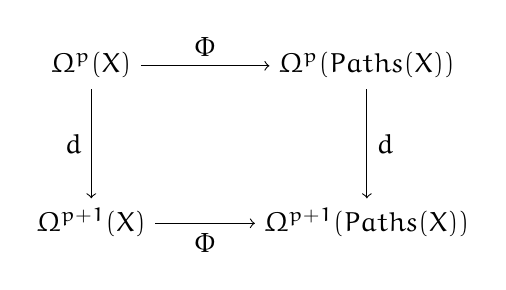
\begin{tikzpicture}[auto]
    \node (A)  at (0,0) {$\DForms^p(\X)$};
    \node (B)  at (3.5,0) {$\DForms^p(\Paths(\X))$};
    \node (C)  at (0,-2) {$\DForms^{p+1}(\X)$};
    \node (D)  at (3.5,-2) {$\DForms^{p+1}(\Paths(\X))$};
    \draw[->] (A) to node {$\Phi$} (B);
    \draw[->] (A) to node [swap] {$d$} (C);
    \draw[->] (B) to node {$d$} (D);
    \draw[->] (C) to node [swap] {$\Phi$} (D);
  \end{tikzpicture}
\end{center}
  \end{article} %% The-operator-Phi-is-a-morphism-of-De-Rham-complex
  
  \begin{proof}
    Let $\alpha$ be a $p$-form on $\X$, $p>0$. Then, with the above notation 
    $\P_t = {\hat t} \circ \P$, where $\P$ is a plot of $\Paths(\X)$, we have:
    \begin{eqnarray*}
      \Phi(d\alpha)(\P) & = &
      \int_0^1 (d\alpha)(\P_t)
      \dt = 
      \int_0^1 d[\alpha(\P_t)] \dt = 
      d \left(\int_0^1 \alpha(\P_t)
      \dt \right)\\
      & = & d (\Phi(\alpha)(\P)).
    \end{eqnarray*}
    Thus, $\Phi(d\alpha) = d(\Phi(\alpha))$.
  \end{proof}
  
  \begin{article}\artlabel{Variance of the integration operator $\Phi$}
    \label{Variance-of-the-integration-operator-Phi}
    Let $\X$ and $\X'$ be two diffeological spaces, let $f:
      \X \to \X'$ be a smooth map. The map $f$ leads to a smooth
    correspondence
    $$
      \fPaths{f}: \Paths(\X) \to \Paths(\X') \quad
      \mbox{with}\quad \fPaths{f}(\gamma) = f \circ \gamma.
      $$
    The map $f$ induces also the two pullbacks:
    $$f^*: \DForms^\star(\X') \to \DForms^\star(\X) \quad
      \mbox{and}\quad  \fPaths{f}^*: \DForms^\star(\Paths(\X'))
      \to \DForms^\star(\Paths(\X)).
      $$
    Let $\Phi_\X$ et $\Phi_{\X'}$, be the two associated
    Integration Operators
    \art{Integration-operator-of-forms-along-paths}, then 
    $$
      \Phi_\X \circ f^* = \fPaths{f}^* \circ \Phi_{\X'}.
      $$
    This is summarized by the following commutative
    diagram.
    \begin{center}
    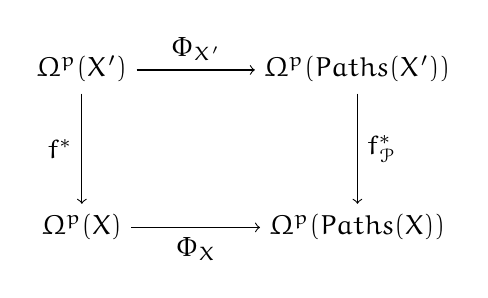
\begin{tikzpicture}[auto]
      \node (A)  at (0,0) {$\DForms^p(\X')$};
      \node (B)  at (3.5,0) {$\DForms^p(\Paths(\X'))$};
      \node (C)  at (0,-2) {$\DForms^p(\X)$};
      \node (D)  at (3.5,-2) {$\DForms^p(\Paths(\X))$};
      \draw[->] (A) to node {$\Phi_{\X'}$} (B);
      \draw[->] (A) to node [swap] {$f^*$} (C);
      \draw[->] (B) to node {$\fPaths{f}^*$} (D);
      \draw[->] (C) to node [swap] {$\Phi_\X$} (D);
    \end{tikzpicture}
\end{center}

  \end{article} %% Variance-of-the-integration-operator-Phi
  
  \begin{proof}
    Let $\alpha$ be a differential $p$-form of $\X'$, and
    $\P: \U \to \Paths(\X)$ be a plot. Let us use the above notation $\P_t =
      {\hat t} \circ \P$, on the one hand we have
    $$
      [(\Phi_\X \circ f^*)(\alpha)](\P) = 
      [\Phi_\X(f^*(\alpha))](\P) =  \int_0^1
      f^*(\alpha)(\P_t) \dt =  \int_0^1 \alpha(f \circ \P_t)
      \dt,
      $$
    and, on the other hand,
    $$
      [(\fPaths{f}^* \circ \Phi_{\X'})(\alpha)](\P) = 
      [\fPaths{f}^*(\Phi_{\X'}(\alpha))](\P) = [\Phi_{\X'}(\alpha)](\fPaths{f} \circ \P) = 
      \int_0^1 \alpha[(\fPaths{f} \circ \P)_t] \dt.
      $$
    But, for any $r \in \U$: 
    $$
      (f \circ \P_t)(r) = f(\P_t(r)) = f(\P(r)(t)),
      $$
    and 
    $$
      (\fPaths{f} \circ \P)_t(r) = (\fPaths{f} \circ
      \P)_t(r) = f(\P(r)(t)).
      $$
    Thus, $f \circ \P_t = (\fPaths{f} \circ \P)_t$, and
    finally:  $\Phi_\X \circ f^* = \fPaths{f}^* \circ
      \Phi_{\X'}$.  \end{proof}
  
  \begin{article}\artlabel{Derivation along time reparametrization}
    \label{Derivation-along-time-reparametrization}
    Let $\X$ be a diffeological space, and let $\Paths(\X)$
    be the space of its smooth paths, equipped with the
    functional diffeology. The group of translations
    $(\RR,+)$ acts smoothly by reparametrization on $\Paths(\X)$, as a
    $1$-parameter group of diffeomorphisms. Let us denote
    by $\tau$ this action. For all $\gamma \in \Paths(\X)$,
    and for  all $e \in \RR$,
    %
    $$ 
      \tau(e): \gamma \mapsto \gamma \circ {\T}_e \quad \mbox{with}
      \quad {\T}_e: t \mapsto t+e.
      $$ 
    Let $\alpha$ be a $p$-form of $\X$, the Lie derivative
    \art{The-Lie-derivative-of-differential-forms} of the
    $p$-form $\Phi(\alpha)$ by the 1-parameter group $\tau$
    satisfies: 
    %
    $$ 
      \DLie_\tau (\Phi(\alpha)) = \but^*(\alpha) -\source^*(\alpha).
      $$ 
  \end{article} %% Derivation-along-time-reparametrization
  
  \begin{proof} Let us check first that $\tau : e \mapsto
    [\gamma \mapsto \gamma \circ \T_e]$ is a smooth
    homomorphism from $(\RR,+)$ into $\Diff(\Paths(\X))$.
    First of all, let us check that $\tau$
    takes its values in $\Diff(\Paths(\X))$: a) For all $e \in
      \RR$, $\tau(e)(\gamma) = \tau(e)(\gamma')$ implies
    $\gamma = \gamma'$, so $\tau(e)$ is injective, and the
    inverse is given by $\tau(e)^{-1} = \tau(-e)$, thus
    $\tau(e)$ is bijective. b) For all $e \in \RR$, $\tau(e)$
    is smooth. Indeed, let $\P$ be a plot of $\Paths(\X)$, that is,
    $(r,t) \mapsto \P(r)(t)$ is a plot of $\X$. Then, 
    $(\tau(e) \circ \P)(r)(t) = (\tau(e)(P(r))(t) = \P(r)(t+e)$, and
    the map $(r,t) \mapsto (r,t+e) \mapsto \P(r)(t+e)$, being a composite of smooth maps, is smooth.
    Thus $\tau(e)$ is smooth, and since $\tau(e)^{-1} = \tau(-e)$, $\tau(e)$ is
    a diffeomorphism of $\Paths(\X)$.
    Next, $\tau$ is clearly an homomorphism, $\tau(e+e') =
      \tau(e) \circ \tau(e')$. Then, let us check that $\tau$ is mooth, that is, $\tau$ is a plot of 
      $\Diff(\Paths(\X))$. The parametrization $\tau$ is a plot of $\Diff(\Paths(\X)$ if and only if
      $(e,\gamma) \mapsto \tau(e)(\gamma)$ and $(e,\gamma) \mapsto \tau(e)^{-1}(\gamma) = \tau(-e)(\gamma)$
       are smooth. That is, for all plots $\P$ of $\Paths(\X)$, if and only if 
       $(e,r) \mapsto \tau(e)(\P(r)) = \P(r)\circ T_e$ is smooth, that is,
       $(e,r,t) \mapsto \P(r)(t+e)$ is smooth,
       which indeed is the case. Thus, $\tau \in \DHom(\RR,\Diff(\Paths(\X)))$.
    
    Now, let us denote $\balpha = \Phi(\alpha)$, we have then, for any plot
    $\P$ de $\Paths(\X)$  
    $$[\DLie_\tau\balpha](\P) = {\partial \over \partial
      t}\bigg\{[\tau(t)^*\balpha](\P)\bigg\}_{t = 0} =
      {\partial \over \partial
      t}\bigg\{\balpha(\tau(t) \circ \P) \bigg\}_{t = 0}.
      $$
    But $\tau(t) \circ \P: r \mapsto \P(r) \circ
      {\T}_t$, thus 
    $$ \balpha [\tau(t) \circ \P] = \int_0^1
      \alpha[(\tau(t) \circ \P)_s] \ds =
      \int_0^1 \alpha[r \mapsto \P(r)(t+s)] \ds.
      $$ 
    Let $u = t+s$, we get 
    $$ 
      \balpha[\tau(t) \circ \P] = \int_t^{1+t} \alpha[r
      \mapsto  \P(r)(u)] \du.
      $$
    After derivation with respect to $t$, for $t = 0$, we get 
    $$[\DLie_\tau\balpha](\P) = \alpha[r \mapsto
      \P(r)(1)] - \alpha[r \mapsto 
      \P(r)(0)] =
      [\but^*\alpha-\source^*\alpha](\P),
      $$ 
     for all plot $\P$ of $\X$. That is $\DLie_\tau (\Phi(\alpha)) = \but^*\alpha
      -\source^*\alpha$. 
  \end{proof}
  
  \begin{article}\artlabel{Variance of the time reparametrization}
    \label{Variance-of-time-reparametrization}
    Let $\X$ and $\X'$ be two diffeological spaces,
    let $f: \X \to \X'$ be a smooth map. Let
    $\fPaths{f}: \Paths(\X) \to \Paths(\X')$ be the action of
    $f$ on paths defined in
    \art{Variance-of-the-integration-operator-Phi} and
    $\fPaths{f}^*: \DForms^p(\Paths(\X')) \to
      \DForms^p(\Paths(\X))$ be the induced action of
    $\fPaths{f}$ at the level of $p$-forms. Let $\tau$ and
    $\tau'$ denote the action $(\RR,+)$ on $\Paths(\X)$ and
    $\Paths(\X')$, as it has been defined in
    \art{Derivation-along-time-reparametrization}. Let
    $i_\tau$ and $i_{\tau'}$ be the contraction associated
    with these $1$-parameter groups of diffeomorphisms
    \art{Contracting-differential-forms-on-sliding}. Then,
    $i_{\tau} \circ \fPaths{f}^* = \fPaths{f}^* \circ
      i_{\tau'}$, summarized by the following
    commutative diagram.
    \begin{center}
    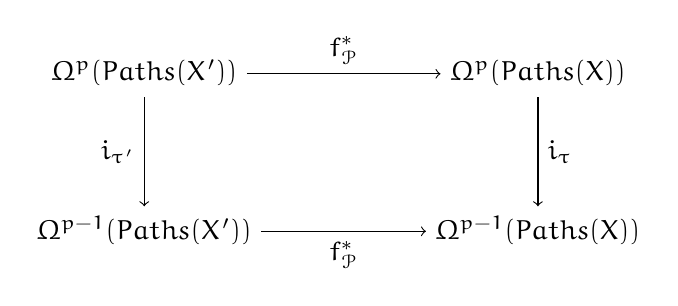
\begin{tikzpicture}[auto]
      \node (A)  at (0,0) {$\DForms^p(\Paths(\X'))$};
      \node (B)  at (5,0) {$\DForms^p(\Paths(\X))$};
      \node (C)  at (0,-2) {$\DForms^{p-1}(\Paths(\X'))$};
      \node (D)  at (5,-2) {$\DForms^{p-1}(\Paths(\X))$};
      \draw[->] (A) to node {$\fPaths{f}^*$} (B);
      \draw[->] (A) to node [swap] {$i_{\tau'}$} (C);
      \draw[->] (B) to node {$i_\tau$} (D);
      \draw[->] (C) to node [swap] {$\fPaths{f}^*$} (D);
    \end{tikzpicture}
    \end{center}
  \end{article} %% Variance-of-time-reparametrization
  
  \begin{proof}
    Let $\beta$ be a $p$-form
    on $\Paths(\X')$, $\P: \U \to \Paths(\X)$ be a $n$-plot,
    $r \in \U$ and $v$ represents $(p-1)$
    vectors of $\RR^n$. By definition of the contraction of a
    $p$-form by a $1$-parameter group of diffeomorphisms
    \art{Contracting-differential-forms-on-sliding}, we have:
    
    1) On the one hand, 
    \begin{eqnarray*}
      [(i_{\tau} \circ \fPaths{f}^*)(\beta)](\P)_r(v)
      & = & [i_{\tau}(\fPaths{f}^*(\beta))](\P)_r(v)
      \\  & = & \fPaths{f}^*(\beta)(\tau\cdot \P)_{0
      \choose r} \begin{pmatrix}1 \\ 0\end{pmatrix} \begin{pmatrix}0 \\ v\end{pmatrix} \\
      & = &
      \beta(\fPaths{f} \circ (\tau\cdot \P))_{0 \choose r}
      \begin{pmatrix}1 \\ 0\end{pmatrix} \begin{pmatrix}0 \\ v\end{pmatrix},
    \end{eqnarray*}
    where
    $\tau\cdot \P(t,r) = \tau(t)(\P(r))$. But, 
    \renewcommand{\theequation}{$\clubsuit$}
    \begin{eqnarray}
      [\fPaths{f} \circ (\tau\cdot \P)](t,r) & = & \fPaths{f}((\tau\cdot
      \P)(t,r)) \nonumber\\ & = & \fPaths{f}(\tau(t)(\P(r)) \nonumber\\ & = &
      \fPaths{f}[s \mapsto \tau(t)(\P(r))(s)]\nonumber\\ & = &
      \fPaths{f}[s \mapsto \P(r)(s+t)] \nonumber\\
      & = & [s \mapsto 
      f(\P(r)(s+t))].
    \end{eqnarray} 
    2) On the other hand,
    \begin{eqnarray*}[(\fPaths{f}^* \circ
      i_{\tau'})(\beta)](\P)_r(v) & = &
      [\fPaths{f}^*(i_{\tau'}(\beta))](\P)_r(v) \\ & =
      & [(i_{\tau'}(\beta)(\fPaths{f} \circ \P)]_r(v)
      \\ & = & \beta(\tau'\cdot(\fPaths{f} \circ \P))_{0 \choose r}
      \begin{pmatrix}1 \\ 0\end{pmatrix} \begin{pmatrix}0 \\ v\end{pmatrix}.
    \end{eqnarray*}
    But,
    \renewcommand{\theequation}{$\spadesuit$}
    \begin{eqnarray}
      [\tau'\cdot(\fPaths{f} \circ \P)](t,r) & = & \tau'(t)(\fPaths{f} \circ \P(r))\nonumber \\
      & = & [s \mapsto (\fPaths{f} \circ \P(r))(s+t)]\nonumber \\
      & = & [s \mapsto f(\P(r)(s+t))]. 
    \end{eqnarray} 
      Now, comparing $(\clubsuit)$ and $(\spadesuit)$, we get
    $$
    [(i_{\tau} \circ \fPaths{f}^*)(\beta)](\P)_r(v) = [(\fPaths{f}^*
      \circ i_{\tau'})(\beta)](\P)_r(v),
      $$
    that is, finally, $i_{\tau} \circ \fPaths{f}^* = \fPaths{f}^*
      \circ i_{\tau'}$.
  \end{proof}
  
  \begin{article}\artlabel{The chain-homotopy operator $\eK$} 
    \label{The-chain-homotopy-operator-K}
    Let $\X$ be a diffeological space. Let $\Phi$ be the
    integration operator defined in
    \art{Integration-operator-of-forms-along-paths},
    let $\tau$ be the time-reparametrization defined in
    \art{Derivation-along-time-reparametrization}, and let
    $i_\tau$ be the contraction by the sliding $\tau$
    \art{Contracting-differential-forms-on-sliding}. The
    operator $\eK: \DForms^p(\X) \to
      \DForms^{p-1}(\Paths(\X))$ defined, for all integer $p>0$, by
    \begin{equation}\tag{$\spadesuit$} 
      \label{defOH}
      \eK =  i_\tau \circ \Phi,
    \end{equation} 
    satisfies  
    \begin{equation}\tag{$\clubsuit$} \label{ophom}
      \eK \circ d +d  \circ \eK =
      \but^* - \source^*.
    \end{equation}
    The operator $\eK$ will be called the {\em
    chain-homotopy operator}. Moreover, $\eK$ is 
    smooth and linear, which is denoted by
    $$
    \eK \in \DLin(\DForms^p(\X), \DForms^{p-1}(\Paths(\X))).
      $$ 
    Let $\alpha \in \DForms^p(\X)$, with $p>1$, for
    $p=1$ see \art{The-Chain-Homotopy-operator-for-p=1}. Let
    $\P : \U \to \Paths(\X)$ be a $n$-plot, the value of
    $\eK\alpha$ on $\P$ is explicitly given by
    $$
      (\eK\alpha)(\P)_r(v_2) \cdots (v_{p}) =
      \int_0^1 \alpha \left[ \begin{pmatrix}s \\ r\end{pmatrix} \mapsto \P(r)(s
      + t) \right]_{0 \choose r} \begin{pmatrix}1 \\ 0\end{pmatrix}
      \begin{pmatrix}0 \\ v_2\end{pmatrix} \cdots \begin{pmatrix}0 \\ v_{p}\end{pmatrix} \dt,
      $$
      where $r \in \U$, and $v_2,\ldots,v_{p}$ are $(p-1)$ vectors of $\RR^n$. 
  \end{article} %% The-chain-homotopy-operator-K
  
  \begin{proof}
    Let $\alpha$ be a $p$-form of $\X$, $p>0$. On the one hand
    \art{Derivation-along-time-reparametrization} we have
    $$\DLie_\tau (\Phi(\alpha)) = \but^*(\alpha) -
      \source^*(\alpha),$$ and on the other hand, applying the
    Cartan formula \art{The-Cartan-Lie-formula} and the
    commutation $d \circ \Phi = \Phi \circ d$
    \art{The-operator-Phi-is-a-morphism-of-De-Rham-complex},
    we get
    \begin{eqnarray*}
      \DLie_\tau (\Phi(\alpha))& =&
      d[i_\tau(\Phi (\alpha))]+i_\tau (d[\Phi (\alpha)]) \\ &=&
      d[i_\tau\Phi (\alpha)]+i_\tau \Phi [d\alpha] \\
      &=& d[\eK(\alpha)] + \eK(d\alpha).
    \end{eqnarray*}
    Hence, $d[\eK(\alpha)] + \eK(d\alpha) = \but^*(\alpha) -
      \source^*(\alpha)$, that is, $\eK \circ d +d  \circ \eK =
        \but^* - \source^*$. Now, because the contraction operation
    and the map
    $\Phi$ 
    are smooth \art{Contraction-of-differential-forms}
    \art{Integration-operator-of-forms-along-paths}, the
    chain-homotopy operator $\eK$ is a smooth linear
    map. The explicit evaluation on the plot $\P$ is a direct
    application of the definitions.
  \end{proof}
  
  \begin{article}\artlabel{The Chain-Homotopy operator for $p = 1$} 
    \label{The-Chain-Homotopy-operator-for-p=1}
    Let $\X$ be a diffeological space. Let $\Paths(\X) =
      \Cinf(\RR,\X)$ be the space of paths of $\X$, equipped
    with the functional diffeology. For every $1$-form
    $\alpha \in \DForms^1(\X)$, $\F_\alpha =  \eK(\alpha)$
    belongs to $\DForms^0(\Paths(\X)) = 
      \Cinf(\Paths(\X),\RR)$, precisely
    $$
      \eK : \DForms^1(\X) \to \Cinf(\Paths(\X),\RR)
      \qmbox{and} \eK(\alpha) = \F_\alpha = \left[
      \gamma \mapsto \int_\gamma\alpha\right].
      $$
    The function $\F_\alpha =
      \eK(\alpha)$ can be extended, by linearity, over the whole
    space $\DChains{1}(\X)$ of $1$-chains of $\X$,
    $$
      \mbox{for
      all } \sum_\gamma n_\gamma \gamma \in \DChains{1}(\X),
      \quad \F_\alpha\bigg(\sum_\gamma n_\gamma \gamma\bigg)
      = \sum_{\gamma} n_\gamma \F_\alpha(\gamma) = 
      \sum_\gamma n_\gamma \int_\gamma \alpha.
      $$
    And thus, for $p = 1$, the
    chain-homotopy operator is just the pairing
    of $1$-forms over $1$-chains. Moreover, if $\gamma$ and
    $\gamma'$ are two paths such that the juxtaposition
    $\gamma\vee\gamma'$ is defined, then
    \begin{equation}
      \renewcommand{\theequation}{$\diamondsuit$}
      \F_\alpha(\gamma\vee\gamma') = \F_\alpha(\gamma +
      \gamma') =  \F_\alpha(\gamma) + \F_\alpha(\gamma').
    \end{equation}
    Note that if the juxtaposition of
    $\gamma$ and $\gamma'$ is not a path, then the
    smashed juxtaposition $\gamma\star\gamma' = 
      \gamma^\star\vee\gamma'$ is a path
    \cite{Piz05}, and satisfies also
    \begin{equation}
      \renewcommand{\theequation}{$\heartsuit$}
      \F_\alpha(\gamma \star\gamma') = \F_\alpha(\gamma +
      \gamma') = \F_\alpha(\gamma) +
      \F_\alpha(\gamma').
    \end{equation}
    In other words,
    $\F_\alpha = \eK(\alpha)$ is a morphism from
    $(\Paths(\X),\star)$ to $(\RR,+)$.
  \end{article} %% The-Chain-Homotopy-operator-for-p=1
  
  \begin{proof}
    If $\gamma\vee\gamma'$ is a path of $\X$, the identity
    $(\diamondsuit)$ is just the additivity of the integral,
    \begin{eqnarray*} 
      \F_\alpha(\gamma\vee\gamma') & = &
      \int_0^1\alpha(\gamma\vee\gamma')(t) \dt \\ 
      & = & \int_0^{1/2}\alpha(s \mapsto \gamma(2s))(t) \dt
      +\int_{1/2}^1\alpha(s \mapsto \gamma'(2s-1))(t) \dt. 
    \end{eqnarray*}
    And, after a suitable change of variable we get
    $$
      \F_\alpha(\gamma\vee\gamma') =
      \int_0^{1}\alpha(\gamma)(t) \dt
      +\int_{0}^1\alpha(\gamma')(t) \dt = \F_\alpha(\gamma) +
      \F_\alpha(\gamma').
      $$
    Now, if we need to smash the paths $\gamma$ and
    $\gamma'$, the proof is the same. It is just the formula
    of change of variable of the integrand,
    $$
      \int_a^b f(\varphi(t)) \varphi'(t) \dt = 
      \int_{\varphi(a)}^{\varphi(b)} f(t) \dt,
      $$ 
    applied to the paths $\gamma^\star = \gamma \circ
      \lambda$ and  $\gamma'^\star = \gamma' \circ \lambda$,
    where $\lambda$ is the smashing
    function described in \cite{Piz05}.
  \end{proof}
  
  \begin{article}\artlabel{The Chain-Homotopy operator for manifolds} 
    \label{The-Chain-Homotopy-operator-for-manifolds}
    Let $\M$ be a manifold of finite dimension. The
    chain-homotopy operator $\eK$
    \art{The-chain-homotopy-operator-K} of $\M$ can be
    expressed using tangent spaces. Let $\P : \U \to
      \Paths(\M)$ be a $n$-plot. Let us denote, for any $r \in
        \U$ and for any vector $\delta_i r \in \RR^n$,
    $$
      \gamma_r
      = \P(r): t \mapsto \gamma_r(t) \quad \mbox{and} \quad \delta
      \gamma_r: t \mapsto \D[r \to \gamma_r(t)](r)(\delta r).
      $$
    Let $\alpha \in
      \Omega^p(\M)$, the real $\eK\alpha(\P)(r)(\delta_2
        r)\cdots(\delta_{p}r)$ can be interpreted as
    $\eK\alpha$, computed at the point $\gamma_r$ and applied
    to the $p-1$ {\em variations} $\delta_i\gamma_r$
    associated to the $p-1$ vectors $\delta_i r$. It can be
    explicited as
    $$ 
      \eK\alpha_{\gamma_r}(\delta_2\gamma_r)\cdots (\delta_{p}
      \gamma_r)
      = \int_0^1\alpha_{\gamma_r(t)}\bigg({d\,\gamma_r(t) \over
      d\,t}\bigg) (\delta_2
      \gamma_r(t))\cdots(\delta_{p}\gamma_r(t))\dt.
      $$ 
  \end{article} %% The-Chain-Homotopy-operator-for-manifolds
  
  \begin{article}\artlabel{Variance of the Chain-Homotopy operator} 
    \label{Variance-of-the-Chain-Homotopy-operator}
    Let $\X$ et $\X'$ be two diffeological spaces. Let
    $f: \X \to \X'$ be a smooth map. Let us use
    the notations of the proposition
    \art{Variance-of-the-integration-operator-Phi} and let
    $\eK_\X$ et $\eK_{\X'}$ be the two chain-homotopy
    operators of $\X$ and $\X'$. Then, the
    variance of the chain-homotopy operators is given by
    $$
      \eK_\X \circ f^* = \fPaths{f}^* \circ \eK_{\X'}.
      $$
    Where $\fPaths{f}$ has been defined in
    \art{Variance-of-the-integration-operator-Phi}, as the
    action of the function $f$ on paths. This is
    summarized by the following commutative diagram.
  \begin{center}
  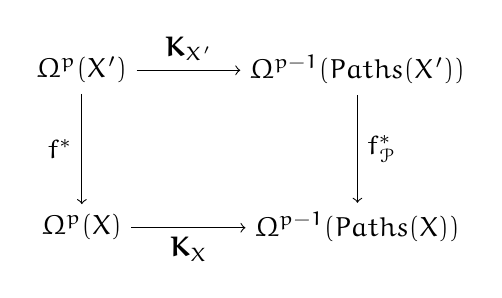
\begin{tikzpicture}[auto]
    \node (A)  at (0,0) {$\DForms^p(\X')$};
    \node (B)  at (3.5,0) {$\DForms^{p-1}(\Paths(\X'))$};
    \node (C)  at (0,-2) {$\DForms^p(\X)$};
    \node (D)  at (3.5,-2) {$\DForms^{p-1}(\Paths(\X))$};
    \draw[->] (A) to node {$\eK_{\X'}$} (B);
    \draw[->] (A) to node [swap] {$f^*$} (C);
    \draw[->] (B) to node {$\fPaths{f}^*$} (D);
    \draw[->] (C) to node [swap] {$\eK_\X$} (D);
  \end{tikzpicture}
\end{center}

  \end{article} %% Variance-of-the-Chain-Homotopy-operator
  
  \begin{proof} Let us denote $\tau$ and $\tau'$ the action
    of $(\RR,+)$ on $\Paths(\X)$ and $\Paths(\X')$ defined in
    \art{Derivation-along-time-reparametrization}. Let
    $\alpha \in \DForms^p(\X')$, by definition
    $\eK_\X(f^*(\alpha)) =  (i_\tau \circ
      \Phi_\X)(f^*(\alpha)) =  i_{\tau}(\Phi_\X(f^*(\alpha)))$,
    but $\Phi_\X \circ f^* =  \fPaths{f}^* \circ \Phi_{\X'}$
    \art{Variance-of-the-integration-operator-Phi}, thus 
    $$
      \eK_\X(f^*(\alpha)) =  i_{\tau}(\Phi_\X \circ
      f^*(\alpha)) =  i_{\tau}(\fPaths{f}^* \circ
      \Phi_{\X'}(\alpha)) = (i_{\tau} \circ
      \fPaths{f}^*)(\Phi_{\X'}(\alpha)).
      $$ 
    Now, thanks to \art{Variance-of-time-reparametrization},
    we have $i_{\tau} \circ \fPaths{f}^* = \fPaths{f}^* \circ
      i_{\tau'}$. Hence, 
    $$
      \eK_\X(f^*(\alpha)) = (\fPaths{f}^* \circ
      i_{\tau'})(\Phi_{\X'}(\alpha)) =  \fPaths{f}^*(i_{\tau'}
      \circ \Phi_{\X'}(\alpha)) = 
      \fPaths{f}^*(\eK_{\X'}(\alpha)).
      $$
    Therefore, $\eK_\X \circ f^* = \fPaths{f}^* \circ
      \eK_{\X'}.$
  \end{proof}
  
  \begin{article}\artlabel{Chain-Homotopy preserves invariance} 
    \label{Chain-Homotopy-preserves-invariance}
    Let $\X$ be a diffeological space and let $\alpha$ be a
    differential $p$-form on $\X$, $p \geq 1$. Let us denote
    by $\Diff(\X,\alpha)$ the group of diffeomorphisms of $\X$
    preserving $\alpha$,
    $$
      \Diff(\X,\alpha) = \{ f \in \Diff(\X) \ \vert \
      f^*(\alpha) = \alpha \}.
      $$
    As an application of the proposition above 
    \art{Variance-of-the-Chain-Homotopy-operator}, we get
    $$
      f \in \Diff(\X,\alpha) \quad \Rightarrow \quad
      \fPaths{f} \in \Diff(\Paths(\X),\eK\alpha). 
      $$ In other words, if a diffeomorphism $f$ of $\X$
    preserves $\alpha$, the action $\fPaths{f}$ of
    $f$ on $\Paths(\X)$ preserves $\eK\alpha$. This property
    is used to construct the moment maps in diffeology
    \cite{Piz07}.
  \end{article} %% Chain-Homotopy-preserves-invariance
  
  %%%%%%%%%%%%%%%%%%%%%%%%%%%%%%%%%%%%%%%%%%%%%%%%%%%%%%%%%%
  %% 
  %% MARK: Homotopy and differential forms, Poincar\'e's lemma
  %%
  %%%%%%%%%%%%%%%%%%%%%%%%%%%%%%%%%%%%%%%%%%%%%%%%%%%%%%%%%%
  
  \section{Homotopy and differential forms, Poincar\'e's lemma} 
  \label{Section-Homotopy-and-differential-forms}
  
  \begin{text}
    One crucial property of the De Rham cohomology, in the general framework of diffeology,
    is its homotopic invariance, proved in this paragraph. That is, the mapping induced
    on the De Rham cohomology by the pullback by a smooth map
    depends only of the homotopy class of the map. The
    equivalent theorem in classical differential geometry,
    for the De Rham cohomology of finite dimensional
    manifolds, can be regarded a specialization of this
    general diffeological result. The transition through the
    space of paths, which is impossible in the restricted
    category of manifolds, offers a great simplification of
    this theorem even for the only case of manifolds.  The
    main tool used in this chapter is the chain-homotopy
    operator defined in the previous chapter
    \art{The-chain-homotopy-operator-K}. This proves by the way, that
    this invariance dwells deeply in the general diffeological structure.
  \end{text}
  
  \begin{article}\artlabel{Homotopic invariance of the De Rham cohomology} 
    \label{Homotopic-invariance-of-the-De-Rham-cohomology}
    Let $\X$ and $\X'$ be two diffeological spaces. Let $s \mapsto f_s$ be
    a smooth path in $\Cinf(\X,\X')$. For all integer $p \geq 1$, for 
    all $\alpha' \in \DForms^p(X')$ such that $d\alpha' = 0$, $f_0^*(\alpha')$ 
    and $f_1^*(\alpha')$ are cohomologous. The case $p=0$ is trivial.
    $$
     \alpha' \in \DForms^p(X') \mbox{ and } d\alpha' = 0 \ \Rightarrow \
     f_1^*(\alpha') = f_0^*(\alpha') + d\beta, \mbox{ with } \beta \in  \DForms^{p-1}(X))
    $$
    Denoting by $f^*_{\rm dR} : \HDR^\star(\X') \to \HDR^\star(\X)$, the action
    of $f \in \Cinf(\X,\X')$ on the De Rham cohomology, the above statement means that
    $f^*_{\rm dR}$ depends only on the homotopy class of $f$ in $\Cinf(\X,\X')$.
  \end{article} %% Homotopic-invariance-of-the-De-Rham-cohomology
  
  \begin{proof}
    Let us consider the following map $\varphi : \X \to \Cinf(\X,\Paths(\X'))$
      $$
      \varphi: x \mapsto [s \mapsto f_s(x)], \qmbox{and} \varphi \in
      \Cinf(\X,\Paths(\X'))
      $$ 
    for the
    functional diffeology. The pullback by $\varphi$ of
    the identity satisfied by the chain-homotopy operator
    $\eK \circ d + d \circ \eK = \but^* - \source^*$ \art{The-chain-homotopy-operator-K} gives:
      $$
        \varphi^*(\eK d \alpha + d\eK \alpha) = \varphi^* (\but^*(\alpha)-\source^*(\alpha)).
      $$ 
Using the hypothesis
    $d\alpha = 0$ and the commutativity between exterior
    differential and pullback
    \art{Exterior-differential-of-forms}, we have on the one
    hand $\varphi^*(\eK d \alpha + d\eK \alpha) = 
      \varphi^*(d\eK \alpha) = d(\varphi^*(\eK\alpha))$, and on the other hand $\varphi^* \circ
      (\but^*-\source^*)(\alpha) = \varphi^* \circ
      \but^*(\alpha)-\varphi^* \circ \source^*(\alpha) =
      (\but\circ\varphi)\,^*(\alpha) -
      (\source\circ\varphi)\,^*(\alpha) = f_1^*(\alpha)-f_0^*(\alpha)$.
    Therefore, $f_1^*(\alpha) =
      f_0^*(\alpha) + d\,\beta$, with $\beta =
        \varphi^*(\eK\alpha)$. 
  \end{proof}
  
  \begin{article}\artlabel{Closed forms on contractible spaces are exact} 
    \label{Closed-forms-on-contractible-spaces-are-exact}
    As a corollary of the above proposition
    \art{Homotopic-invariance-of-the-De-Rham-cohomology}, we
    deduce that every closed form on a contractible
    diffeological space $\X$ is exact, where {\em contractible} means 
    (smoothly) homotopy equivalent to a point. This is the diffeological variant
    of a classic theorem due to Poincar\'e.
  \end{article} %% Closed-forms-on-contractible-spaces-are-exact
  
  \begin{proof}
    Let $\rho$ be a {\em deformation retraction} from a
    diffeological space $\X$ to a point $x_0$. That is,
    $$\rho \in \Paths(\Cinf(\X,\X)) \quad \mbox{such
      that} \quad \rho(0) = [x \mapsto x_0]
      \quad\mbox{and}\quad\rho(1) = \id_\X.$$ With the
    above notations 
    \art{Homotopic-invariance-of-the-De-Rham-cohomology},
    for any closed $p$-form $\alpha$: 
    $$
      \rho(1)^*(\alpha) =
      \rho(0)^*(\alpha) + d\beta,
      $$
    but
    $\rho(1)^*(\alpha) = \alpha$ and
    $\rho(0)^*(\alpha) = [x \mapsto 
      x_0]^*(\alpha) = 0$, and thus $\alpha = d\,\beta$.
  \end{proof}
  
  \begin{article}\artlabel{Closed forms on centered paths spaces}
    \label{Closed-forms-on-centered-paths-spaces}
    Let $\X$
    be a diffeological space and $x_0 \in \X$ be some point.
    Let $\Paths(\X,x_0,\star)$ be the subspace of paths in
    $\X$, {\em centered at $x_0$\/}, that
    is the subspace of paths $\gamma$ in $\X$ such that $\gamma(0) = x_0$. 
    This space is contractible,
    the map $\rho = s \mapsto [\gamma \mapsto 
      [\gamma_{s}: t \mapsto  \gamma(st)]]$ is a deformation
    retraction from
    $\Paths(\X,x_0,\star)$ to the constant path $[t
      \mapsto x_0]$. Therefore, any closed form on
    $\Paths(\X,x_0,\star)$ is exact
    \art{Closed-forms-on-contractible-spaces-are-exact}. That
    is, $\HDR^0(\Paths(\X,x_0,\star)) = \RR$ and 
    $\HDR^p(\Paths(\X,x_0,\star)) = 0$, for all $p>0$. This
    fact is used to construct geometrical realizations (as
    diffeological fiber bundles with connections) of closed
    1-forms and 2-forms, see \cite{Piz05}.
  \end{article} %% Closed-forms-on-centered-paths-spaces
  
  \begin{article}\artlabel{The Poincar\'e lemma} 
    \label{The-Poincare-lemma}
    Let $\X$ be a diffeological space. As a corollary of 
    \art{Closed-forms-on-contractible-spaces-are-exact}, if
    $\X$ is locally contractible \cite{Piz05}
    then any closed $p$-form $\alpha$, $p>0$, is locally exact.
    That is for each point $x \in \X$ there exists a D-open
    neighborhood $\U$ of $x$, and a
    $(p-1)$-form $\beta$, defined on $\U$, such that
    $\alpha\restriction \U = d\beta$. This proposition
    extends Poincar\'e's lemma about integration of closed
    forms on star-shaped domains. It applies on a
    lot of diffeological spaces, in particular it apply on some
    diffeological manifolds \cite{Piz06-b}.
    
    {\sc Note.} As a corollary, since manifolds are
    locally diffeomorphic to $\RR^n$ they are
    locally contractible, and closed forms are locally exact, as we know. 
    But this is not anymore the
    case in diffeology in general, for example the irrational tori
    \cite{Piz05} where every form is closed but not exact or locally exact.
  \end{article} %% The-Poincare-lemma
	
	%%%%%%%%%%%%%%%%%%%%%%%%%%%%%%%%%%%%%%%%%%%%%%%%%%%%%%%%%%
	%% 
	%% MARK: Bibliography
	%% 
	%%%%%%%%%%%%%%%%%%%%%%%%%%%%%%%%%%%%%%%%%%%%%%%%%%%%%%%%%%
	
  %%%%%%%%%%%%%%%%%%%%%%%%%%%%%%%%%%%%%%%%%%%%%%%%%%%%
  % La bibliographie 
  %%%%%%%%%%%%%%%%%%%%%%%%%%%%%%%%%%%%%%%%%%%%%%%%%%%%
  
  \begin{thebibliography}{Piz07-b}
    
    \bibitem[Che77]{Che77}
    \newblock{Kuo Tsai Chen.}
    \newblock{\em Iterated path integrals.}
    \newblock{Bull. of Am. Math. Soc.}
    \newblock{vol. 83,}
    \newblock{no. 5,}
    \newblock{pp.~831--879,}
    \newblock{1977.}
    
    \bibitem[Don84]{Don84}
    \newblock{Paul Donato.}
    \newblock {\em Rev\^etement et groupe fondamental des espaces diff\'e\-rentiels homog\`enes.}
    \newblock {Doctorate dissertation, Universit\'e de Provence, Marseille, 1984.}

    \bibitem[Don94]{Don94}
    \newblock{Paul Donato}
    \newblock{\em $\rm{Diff}(\S^1)$ as coadjoint orbit in the Virasoro space of moments.}
    \newblock{Journal of Geometry and Physics,}
    \newblock{vol. 13,}
    \newblock{pp. 299--305,}
    \newblock{1994.}
    
    \bibitem[DI85]{DI85}
    \newblock{Paul Donato and Patrick Iglesias.}
    \newblock{\em Exemple de groupes diff\'eo\-lo\-gi\-ques : flots irrationnels sur le tore.}
    \newblock{Compte Rendu de l'Acad\'emie des Sciences,}
    \newblock{vol. 301,}
    \newblock{no 4,}
    \newblock{1985.}
    
    \bibitem[Igl85]{Igl85}
    \newblock{Patrick Iglesias}
    \newblock {\em Fibr\'es diff\'eologiques et homotopie.}
    \newblock {Doctorate dissertation, Universit\'e de Provence, Marseille, 1985.}
    
    \bibitem[Igl86]{Igl86}
    \newblock{Patrick Iglesias}
    \newblock{\em Diff\'eologie d'espace singulier et petits diviseurs.}
    \newblock{Compte Rendu de l'Acad\'emie des Sciences,}
    \newblock{vol. 302,}
    \newblock{pp. 519--522,}
    \newblock{1986.}
    
    \bibitem[Igl87]{Iglesias2bis}
    \newblock{Patrick Iglesias}
    \newblock{{\em Connexions et diff\'eologie}}
    \newblock{In ``Aspects dynamiques et topolo\-gi\-ques des groupes infinis de 
    transformation de la m\'ecanique'',}
    \newblock{vol. 25,}
    \newblock{pp. 61--78.}
    \newblock{Hermann, Paris, 1987.}
    
    \bibitem[Igl95]{Igl95}
    \newblock{Patrick Iglesias}
    \newblock {\em La trilogie du Moment.}
    \newblock {Ann. Inst. Fourier,}
    \newblock{vol. 45, no 3, pp.~825--857,}
    \newblock{1995.}
    
    \bibitem[IL90]{IglLac90}
    \newblock{Patrick Iglesias and Gilles Lachaud.} 
    \newblock{\em Espaces diff\'erentiables singuliers et corps de nombres alg\'ebriques.}
    \newblock{Ann. Inst. Fourier, Grenoble,}
    \newblock{vol. 40,}
    \newblock{no 1,}
    \newblock{pp. 723--737,}
    \newblock{1990.}
    
    \bibitem[Piz05]{Piz05}
    \newblock{Patrick Iglesias-Zemmour.} 
    \newblock{\em Diffeology.}
    \newblock{eprint, 2005 --- 2009.}
    \newline
    \newblock{Url: {\tt http://math.huji.ac.il/$\sim$piz/diffeology/}}
    
    \bibitem[Piz06]{Piz06}
    \newblock{Patrick Iglesias-Zemmour.} 
    \newblock{\em Dimension in diffeology.}
    \newblock{Indagationes Mathematicae,}
    \newblock{vol. 18,}
    \newblock{no 4,}
    \newblock{2007.}
    
    \bibitem[Piz06-b]{Piz06-b}
    \newblock{Patrick Iglesias-Zemmour.} 
    \newblock{\em Diffeology of the Infinite Hopf Fibration}
    \newblock{In ``Geometry and Topology of Manifolds''.}
    \newblock{Polish Academy of Sciences,}
    \newblock{Banach Center Publications,}
    \newblock{vol. 76,}
    \newblock{Warszawa, 2007.}
    
    \bibitem[Piz07]{Piz07}
    \newblock{Patrick Iglesias-Zemmour.} 
    \newblock{\em The moment maps in diffeology.}
    \newblock{Memoirs of the AMS,}
    \newblock{vol 972,}
    \newblock{2010.}
    \newline
    \newblock{Url: {\tt http://math.huji.ac.il/$\sim$piz/documents/TMMID.pdf}}
    
    \bibitem[IKZ05]{IKZ05}
    \newblock{Patrick Iglesias, Yael Karshon and Moshe Zadka.} 
    \newblock{\em Orbifolds as diffeologies.}
    \newblock{Transaction of the American Mathematical Society,}
    \newblock{vol. 362,}
    \newblock{no 6,}
    \newblock{pp. 2811--2831,}
    \newblock{2010}
    
    \bibitem[Sou81]{Sou81}
    \newblock{Jean-Marie Souriau.}
    \newblock{\em Groupes diff\'erentiels.}
    \newblock{In ``Lecture notes in mathematics'',}
    \newblock{vol. 836,}
    \newblock{pp. 91--128,}
    \newblock{Springer Verlag, New-York,}
    \newblock{1981.}
    
    \bibitem[Sou84]{Sou84}
    \newblock{Jean-Marie Souriau.}
    \newblock{\em Groupes diff\'erentiels et physique math\'ematique.}
    \newblock{In ``Group Theoretical Methods in Physics'',}
    \newblock{col. Travaux en cours,}
    \newblock{vol. 201,}
    \newblock{pp.~73--119,}
    \newblock{Hermann, Paris}
    \newblock{1984}
    
  \end{thebibliography}
  
  %%%%%%%%%%%%%%%%%%%%%%%%%%%%%%%%%%%%%%%%%%%%%%%%%%%%
  % Signature 
  %%%%%%%%%%%%%%%%%%%%%%%%%%%%%%%%%%%%%%%%%%%%%%%%%%%%
  
  \bigskip
  \flushright{Completed at \\ The Hebrew University of Jerusalem
  \\ Einstein Institute, Campus Givat Ram \\
  Jerusalem 91904, Israel }
  
	
\end{document}
